\chapter{Fundamentals}
In this chapter, we embark on a journey to construct the narrative foundation that underpins our
thesis. Here, we will introduce the essential design concepts and the architectural principles that
have been employed in the creation of the platform known as Kube. Central to this discussion is
cloud computing, which serves as the bedrock for the platform's operational environment. We then
navigate through the intricacies of microservices, an architectural style that breaks down
applications into smaller, independently deployable services. A pivotal aspect of Kube's
architecture is its serverless framework, which facilitates greater scalability and efficiency.
Complementing this is the implementation of sagas, a sequence of transactions that manage failures
and ensure data consistency across services. Lastly, the event-driven architecture of Kube plays a
crucial role, enabling reactive programming and responsive interactions within the platform.
Together, these concepts embody the architectural design of Kube, prioritizing flexibility,
scalability, and robust service integration.

\section{Cloud Computing}
The advent of cloud computing has revolutionized the way we approach computing and data management.
This section of the thesis will explore the paradigm of cloud computing, which has emerged as a
transformative force in the technological landscape. We will examine the fundamental aspects of
cloud computing, including its service models, deployment strategies, and the pivotal role it plays
in modern IT infrastructure.

\subsection{Definition}
The United States National Institute of Standards and Technology's definition of cloud computing
is\textsuperscript{\cite{nist}}:

\begin{quote}
    Cloud computing is a model for enabling ubiquitous, convenient, on-demand network access to a
    shared pool of configurable computing resources (e.g., networks, servers, storage, applications, and
    services) that can be rapidly provisioned and released with minimal management effort or service
    provider interaction. This cloud model is composed of five essential characteristics, three service
    models, and four deployment models.
\end{quote}

Cloud computing offers a highly flexible service delivery model, enabling on-demand access to
various resources, such as storage, processing power, and applications, via the internet. This
eliminates the need for local servers, shifting data handling to online remote servers and offering
a cost-effective, pay-for-what-you-use pricing model. Services like Amazon Web Services (AWS)
provide the technology infrastructure, allowing users to scale operations with ease. Additionally,
this model promotes economic efficiency, as organizations pay only for resources they consume,
supporting a scalable and agile approach to resource management. The network, often the internet,
serves as a conduit between users and cloud services, ensuring data is managed with strong security
measures.

\subsubsection{Essential Characteristics}
Five essential characteristics of cloud computing are\textsuperscript{\cite{nist}}:
\begin{itemize}
    \item \textbf{On-Demand Self-Service}: Users can independently set up and manage their computing needs, such as
          server time and network storage, automatically, eliminating the need for direct interaction with
          service providers.
    \item \textbf{Broad Network Access}: Services are accessible over the internet using standard methods that
          support a diverse range of devices, including smartphones, tablets, laptops, and desktops.
    \item \textbf{Resource Pooling}: The provider's computing resources are aggregated to serve various customers
          under a multi-tenant model. Resources are dynamically allocated and reallocated based on user
          demand, with the user typically not knowing or controlling the exact physical location of the
          resources but may be able to designate a location at a broader level (such as country, state, or
          data center).
    \item \textbf{Rapid Elasticity}: Services can be quickly scaled up or down to match demand, with the scaling
          process sometimes occurring automatically. From the user's perspective, the supply of available
          resources often seems boundless and can be acquired in any volume at any time.
    \item \textbf{Measured Service}: Cloud platforms automatically monitor, control, and report resource usage with
          a metering function that operates at an appropriate level of detail, depending on the type of
          service, such as storage space, processing power, bandwidth, or active user numbers. This metering
          provides clear visibility into the usage of services for both the provider and the consumer.
\end{itemize}

\subsection{Service Models}
Cloud computing has revolutionized the way businesses approach technology, offering a spectrum of
services that cater to varying requirements for control, flexibility, and management. As
organizations transition to cloud-based solutions, understanding the different service models
becomes crucial for leveraging the full potential of the cloud.

The figure \ref{fig:3_cloud_models} shows the three primary cloud service models, forming what is
often referred to as the cloud computing "stack," include Infrastructure as a Service (IaaS),
Platform as a Service (PaaS), and Software as a Service (SaaS). These service models are designed to
build upon one another, offering layers of abstraction and increasing levels of managed
services\textsuperscript{\cite{cloud_amazon}}.

\begin{figure}
    \centering
    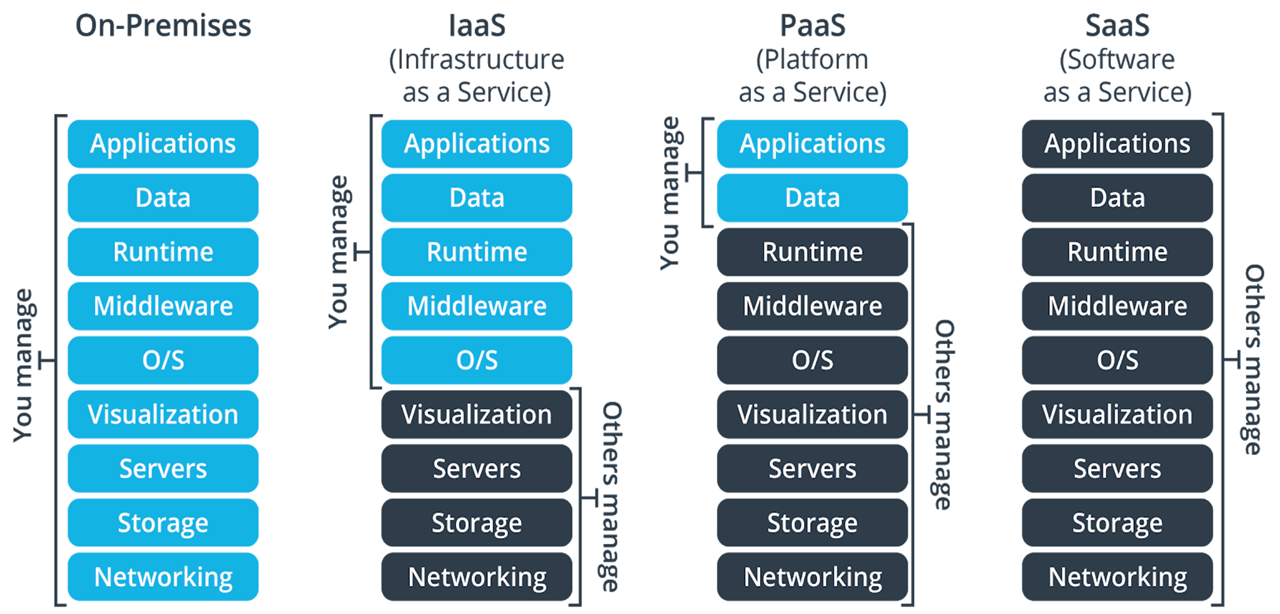
\includegraphics[scale=0.25]{Pictures/3_cloud_models.png}
    \caption{Cloud service models \textsuperscript{\cite{cloud_models}}.}
    \label{fig:3_cloud_models}
\end{figure}

\subsubsection{Infrastructure as a Service (IaaS)}
Infrastructure as a Service (IaaS) is a transformative approach to managing IT resources, offering
flexible and on-demand access to essential infrastructure services through the internet. This
includes virtual machines, storage, and networking that can be customized and billed based on actual
usage. IaaS grants organizations unprecedented control over their IT resources, closely resembling
traditional on-premises infrastructure. It allows for easy scalability without the need for costly
upfront investments in hardware. IaaS empowers consumers with the ability to provision processing,
storage, and networking resources, deploying and running various software, including operating
systems and applications. This level of customization enables organizations to tailor their IT
environment to their specific needs, ensuring a seamless and efficient operation in the cloud.

\subsubsection{Platform as a Service (PaaS)}
Platform as a Service (PaaS) is a significant innovation in cloud computing, offering comprehensive
hardware and software resources for cloud-based application development. Leading PaaS providers
simplify development by effectively managing the underlying infrastructure, allowing a laser focus
on application creation. With PaaS, you're free from infrastructure oversight, enabling dedicated
attention to application deployment and management, improving operational efficiency by eliminating
resource provisioning, capacity planning, and maintenance. PaaS provides an environment for
building, testing, and managing software applications without the need to manage the underlying
cloud infrastructure. As a user, you control your applications and their hosting settings,
simplifying the development process by allowing you to focus solely on creating and deploying your
applications.

\subsubsection{Software as a Service (SaaS)}
Software as a Service (SaaS) is a cloud computing model that delivers software applications over the
internet on a subscription basis. In this approach, cloud providers manage and host the
applications, ensuring their availability, performance, and security. Well-known examples of SaaS
offerings include Google Workspace, Microsoft Office 365, and Salesforce. SaaS provides a complete
software solution over the internet, including the application and its underlying infrastructure,
which is fully maintained by the cloud service provider. This approach spares users from managing
the infrastructure, as the provider handles software updates and security measures. Users can access
these applications through different devices and web browsers, enjoying an accessible and simplified
experience. SaaS enables users to efficiently utilize applications hosted on the cloud, focusing
solely on using the software rather than its maintenance.

\subsection{Deployment Models}
% possibile immagine da qui https://www.slideteam.net/cloud-computing-deployment-models-cloud-service-models-it.html
Cloud computing, a key driver in modern IT resource management, offers various deployment models
tailored to different business needs, security requirements, and scalability demands. This
exploration focuses on Public, Private, Hybrid, and Community Cloud models, discussing their unique
features, benefits, and considerations.

\subsubsection{Community Cloud}
Community-dedicated cloud infrastructure is exclusively used by a specific community of
organizations with shared interests, including mission objectives, security requirements, policies,
and compliance regulations. This infrastructure can be managed by one or more organizations within
the community, external providers, or a combination of both, and it can be located on-premises or
off-premises to accommodate community preferences\textsuperscript{\cite{nist}}.

\subsubsection{Private Cloud}
A private cloud is a form of cloud computing providing exclusive resources and services via a
private network, dedicated solely to one organization. It offers enhanced security and data
isolation, with the ability to tailor infrastructure and software to specific needs and workflows.
While offering robust security and control, private clouds can be costlier due to the organization's
responsibility for infrastructure management and scaling. These can be deployed on-site or hosted by
third-party providers, catering specifically to businesses requiring high security and compliance
standards. The combination of cloud computing benefits with heightened data security and
customization makes private clouds an attractive option for businesses handling sensitive data.

\subsubsection{Public Cloud}
In public cloud computing, a third-party service provider manages all the level of infrastructure,
including servers, storage, and computing resources. Clients access these resources via the internet
and are billed based on their actual usage, creating a cost-effective and flexible pay-as-you-go
model. These cloud environments eliminate the need for substantial investments in expensive
infrastructure, democratizing access to cloud computing. It's important to note that public clouds
operate on shared infrastructure, which offers cost efficiencies but raises concerns about data
isolation and privacy, as multiple customers' data and applications coexist on the same
infrastructure.

\begin{figure}
    \centering
    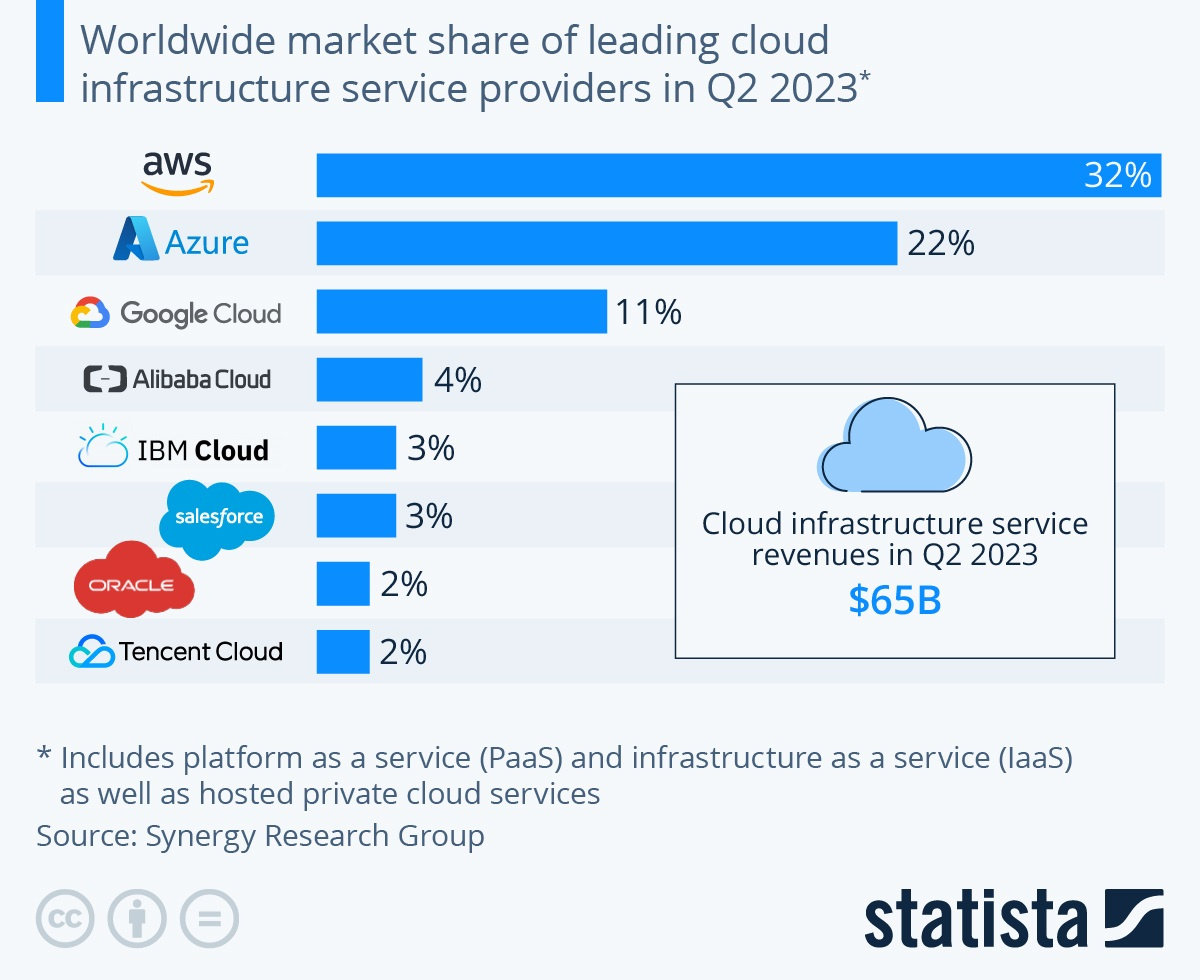
\includegraphics[scale=0.25]{Pictures/3_cloud_vendors.png}
    \caption{Worldwide market share of leading cloud infrastructure service providers in Q2 2023\textsuperscript{\cite{market_cloud_vendors}}.}
    \label{fig:3_cloud_vendors}
\end{figure}

The figure \ref{fig:3_cloud_vendors} show how the public cloud marketplace consists of numerous
cloud providers. Amazon, Microsoft and Google account for 65\% of the total 2023 cloud market. The
remaining public cloud market is divided among IBM, Alibaba, Oracle and several smaller players. The
table \ref{tab:cloud_providers} make a comparison between the major cloud providers.

\begin{table}
    \centering
    \begin{tabular}{|l|c|p{3.8cm}|p{3.8cm}|}
        \hline
        \textbf{Name}            & \textbf{Cost/hour} & \textbf{Pros}                              & \textbf{Cons}                                            \\ \hline
        \textbf{Amazon AWS}      & \$0.0255           & Reliability, Quality, Professional Support & Expensive despite regular lowering of price              \\ \hline
        \textbf{Google GCP}      & \$0.0475           & Reliability, Affordable                    & Limited features and services                            \\ \hline
        \textbf{Microsoft Azure} & \$0.043            & Best infrastructure configuration          & Unsatisfactory customer experience and technical support \\ \hline
        \textbf{IBM Cloud}       & \$0.04             & Flexibility, Speed, Interoperability       & Complicated pricing model and platform can be slow       \\ \hline
    \end{tabular}
    \caption{Comparative overview of major cloud service providers\textsuperscript{\cite{top_cloud_vendors}}.}
    \label{tab:cloud_providers}
\end{table}

\subsubsection{Hybrid Cloud}
The hybrid cloud is an advanced cloud computing model that blends public and private clouds, giving
organizations the flexibility to distribute their applications and workloads as needed. This setup
allows for greater control and scalability than using only public clouds, letting businesses keep
sensitive data secure while still enjoying public cloud efficiency. It's ideal for companies that
need both strong security and the ability to quickly adapt and scale. The hybrid cloud offers a
versatile IT infrastructure that adjusts to the complex needs of modern businesses, improving
security, compliance, and overall efficiency. This makes it a valuable asset for companies
navigating the rapidly changing digital world.

\subsection{Benefits}
Cloud computing is a big shift from the traditional way businesses think about IT resources. Here
are seven common reasons organizations are turning to cloud computing services\textsuperscript{\cite{cloud_azure}}:

\begin{itemize}
    \item \textbf{Cost}: Cloud computing reduces the capital expense of buying hardware and
          software, setting up and running on-site datacenters, which can quickly add up.
    \item \textbf{Speed}: Cloud services are typically on-demand, allowing vast amounts of computing
          resources to be provisioned in minutes, offering businesses flexibility and easing capacity
          planning.
    \item \textbf{Global Scale}: It includes the ability to elastically scale IT resources,
          providing the right amount of computing power, storage, and bandwidth when and where needed.
    \item \textbf{Productivity}: Cloud computing eliminates many time-consuming tasks associated
          with managing on-site datacenters, allowing IT teams to focus on more important business goals.
    \item \textbf{Performance}: Cloud services run on a worldwide network of secure datacenters,
          regularly upgraded to the latest generation of fast and efficient computing hardware, offering
          benefits like reduced network latency and greater economies of scale.
    \item \textbf{Reliability}: Data backup, disaster recovery, and business continuity are easier
          and less costly, as data can be mirrored at multiple redundant sites on the cloud provider’s
          network.
    \item \textbf{Security}: Cloud providers typically offer a broad set of policies, technologies,
          and controls to strengthen security, protecting data, apps, and infrastructure from threats.
\end{itemize}

\subsection{Market Overview}
The global cloud computing market, valued at USD 483.98 billion in 2022, is expected to exhibit a
robust compound annual growth rate (CAGR) of 14.1\% from 2023 to
2030\textsuperscript{\cite{market_cloud_computing}}. This remarkable growth is attributed to the
cloud's capacity to significantly enhance business performance in large enterprises, the increasing
demand for hybrid and Omni-cloud systems, and the adoption of pay-as-you-go models. Cloud services
have gained popularity in developing countries, thanks in part to government initiatives aimed at
safeguarding data integrity and security. The COVID-19 pandemic has expedited the adoption of cloud
computing, driven by the shift towards hybrid work models. While data privacy and security concerns
remain, large enterprises are increasingly turning to cloud-based technologies to optimize costs.
Moreover, cloud adoption is on the rise among small and medium-sized organizations, and governments
in developing nations are making substantial investments in cloud delivery models to enhance
productivity. The Figure \ref{fig:3_cloud_computing_market} illustrates the growth of the U.S. cloud
computing market.

\begin{figure}
    \centering
    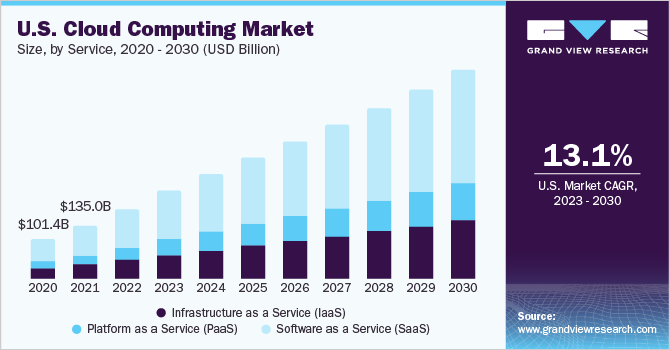
\includegraphics[scale=0.5]{Pictures/3_cloud_computing_market.png}
    \caption{U.S. cloud computing market\textsuperscript{\cite{market_cloud_computing}}.}
    \label{fig:3_cloud_computing_market}
\end{figure}

\section{Microservices}
This section of the thesis is dedicated to a comprehensive exploration of microservices as an
architectural choice that has seen an increasingly popularity over the past half-decade. It aims to
unpack the intricacies of microservices, given a broad overview of the core ideas behind this technology and some
reasons why these architectures are used so widely.

\subsection{Characteristics}
Microservices architecture is a modular approach to software development, breaking complex
applications into smaller, independent components—microservices—tailored to specific business
domains like inventory management or order processing. These microservices, with well-defined
interfaces, can be developed and deployed independently, ensuring flexibility and the evolution of
each component without affecting others. This architecture supports a service-oriented approach,
emphasizing independent deployability and technology neutrality, suitable for diverse technical
challenges\textsuperscript{\cite{microservices_book}}.
\newline\newline
Internally, microservices encapsulate their functionality, operating via network endpoints and
hiding implementation details like programming languages or data storage. This ensures effective
complexity management, with each service maintaining its own data storage, avoiding shared database
issues.
\newline\newline
Externally, microservices act as 'black boxes,' offering functionality without exposing internal
processes. This approach protects against impacts from internal changes, as long as interfaces
remain compatible. It enables seamless updates and maintenance, supporting independent development
and continuous integration.
\newline\newline
Key characteristics of microservices include loose coupling for flexibility and high cohesion for
maintainability. They allow targeted scalability, parallel team work, and robust security, with each
service secured separately. This makes microservices ideal for creating adaptable, scalable, and
sustainable software in rapidly evolving business and technology environments.

\subsubsection{Microservices in the Context of Cloud Computing}
The integration of microservices and cloud computing marks a significant progression in software
architecture, fostering dynamic, scalable, and resilient systems. The decentralized nature of
microservices aligns seamlessly with cloud environments, providing agility and scalable
infrastructure to meet varying service demands. Cloud platforms enhance resource optimization,
ensuring efficient and cost-effective operations. This synergy enables organizations to exploit
cloud computing's robustness, supporting microservices' complex interactions for heightened
scalability and resilience. It allows for continuous integration and deployment, promoting rapid
innovation. Additionally, strategic distribution of microservices across various regions in the
cloud enhances fault tolerance and ensures a consistent user experience globally.

\subsubsection{Example of a Microservice Architecture}
A prime example of microservices in action is the streaming giant Netflix, which has become
synonymous with the successful implementation of this architectural style. The backend architecture
of Netflix, a detailed account of which is provided in an article on
DEV.to\textsuperscript{\cite{microservice_example}}, is a testament to the company's innovative
engineering approach.

\begin{figure}
    \centering
    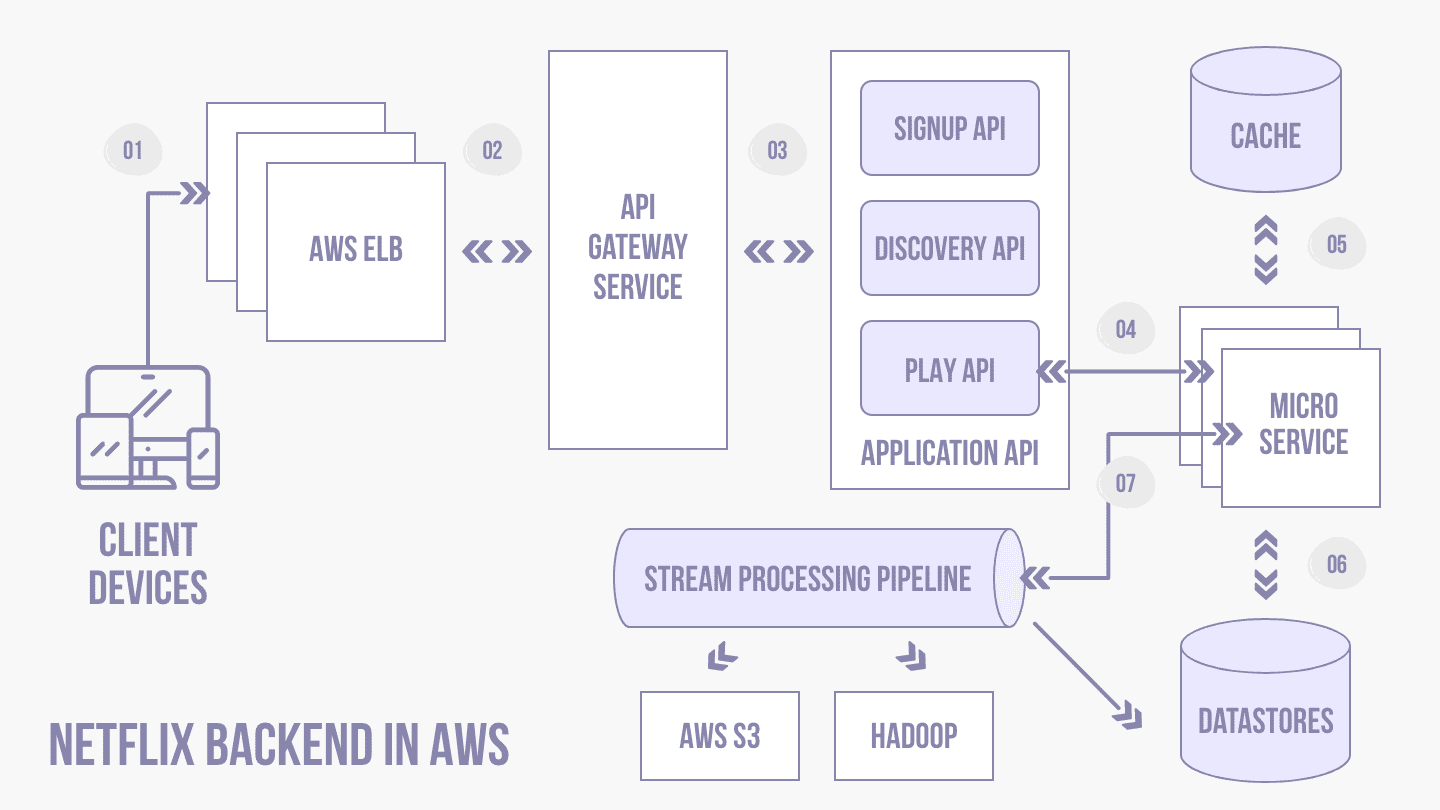
\includegraphics[scale=0.25]{Pictures/3_netflix.png}
    \caption{Netflix backend in AWS\textsuperscript{\cite{microservice_example_image}}.}
    \label{fig:3_netflix}
\end{figure}

How we can see in Figure \ref{fig:3_netflix}, Netflix's backend is a conglomeration of microservices
that operate on Amazon Web Services (AWS), enabling them to serve a staggering amount of content
globally with high availability and resilience. Each microservice is designed to perform a specific
function, such as handling login requests, processing user recommendations, or managing customer
support interactions. This division of responsibilities allows for independent scaling and
development of services, which is crucial given the diversity of Netflix's content and the
variability in demand. The microservices architecture is not only a core component of their backend
system but also underpins their Open Connect content delivery network (CDN), ensuring optimal
streaming performance by placing servers within Internet Service Provider (ISP) networks around the
world. This architecture facilitates rapid and reliable delivery of complex applications at scale,
illustrating the microservices model's capacity to support large-scale enterprise systems
efficiently and effectively.

\newpage

\subsection{Benefits}
This section delves into the multifaceted advantages of adopting microservices. From enhanced
scalability to independent deployment cycles, microservices promise a range of benefits that cater
to both technical and business needs. By dissecting these advantages, this section aims to elucidate
why microservices are becoming the architectural choice for many modern enterprises, providing them
with the flexibility and agility required to thrive in a competitive
market\textsuperscript{\cite{microservices_gitlab}}.

\subsubsection{Scalability}
Microservices excel in scalability due to their ability to be scaled individually. This granular
scalability allows for precise allocation of resources to different components based on fluctuating
demands, leading to enhanced efficiency in resource utilization. Unlike monolithic architectures,
where scaling often requires scaling the entire application, microservices operate independently.
This independence facilitates the seamless addition, removal, updating, or scaling of each service
without causing interruptions to the rest of the system. Organizations benefit from this by being
able to dynamically allocate resources to microservices experiencing spikes in demand—such as during
peak shopping seasons—and similarly, scale them down when demand wanes, thereby optimizing the use
of resources and computing power across the service landscape.

\subsubsection{Robustness}
Microservices architecture enhances the robustness of software applications by leveraging its
inherent decoupling. Individual services can fail without precipitating a system-wide shutdown,
thereby preventing a single point of failure from causing cascading breakdowns. In comparison,
monolithic architectures are susceptible to the domino effect, where a single component's failure
can paralyze the whole application. Microservices inherently design for failure, allowing the system
to degrade gracefully and maintain functionality even when certain services are down. However,
network and machine failures are inevitable, and strategies must be in place to handle these
incidents without significantly affecting the user experience.

\subsubsection{Technology agnostic}
Microservices architecture stands out for its technological flexibility, granting teams the liberty
to select the most suitable technology stack for each distinct service. This technology-agnostic
approach decouples services from any singular, early-stage technology decisions that often constrain
entire projects. Within this paradigm, each microservice can be developed using different
programming languages and data storage solutions, according to what best serves its purpose. This
not only streamlines development by aligning with teams' existing proficiencies but also avoids the
overhead of learning new languages unnecessarily. For instance, organizations like Netflix and
Twitter predominantly utilize the Java Virtual Machine (JVM) as their operational platform
\textsuperscript{\cite{microservices_book}}. Their choice is driven by a deep familiarity with this
technology.

\subsubsection{Distributed Development}
Microservices architecture allows development teams to independently build, deploy, and manage their
services, speeding up updates and feature additions with minimal disruption to the overall system.
This facilitates swift adaptation to changing business needs. Unlike monolithic applications, which
require large-scale deployments for minor updates, microservices support targeted, independent
changes to specific services. This reduces deployment risks, enables quick error recovery, and
hastens the delivery of new features to customers. Companies like Amazon and Netflix leverage
microservices to bypass obstacles in software delivery, ensuring rapid and reliable service to their
users\textsuperscript{\cite{microservices_book}}.

\subsubsection{Team optimization}
Microservices architecture enhances team productivity by adhering to the "two-pizza rule," where
smaller teams—ideally just large enough to be fed with two pizzas—tend to produce higher quality
outcomes due to improved focus and manageability. This approach, pioneered by Amazon, ensures that
each team works on a discrete codebase, fostering efficiency and faster achievement of goals. The
flexibility inherent in microservices also allows for easy reassignment of service ownership,
facilitating a seamless adaptation of the architecture to align with evolving organizational
structures, thereby maintaining efficiency and effectiveness in the long term.


\subsection{Challenges}
While the microservices architecture offers numerous benefits such as enhanced scalability and
improved team productivity, it also introduces a set of challenges that can complicate system design
and maintenance: the complexity of orchestrating numerous services, maintaining data consistency
across distributed systems and managing inter-service communication efficiently. Addressing these
challenges is essential for a smooth microservices architecture.

\subsubsection{Complexity}
The decentralized approach of microservices inherently leads to systems with a high degree of
complexity. As the number of services increases, the overall system can become more challenging to
oversee and manage. Debugging exemplifies this complexity; with each microservice generating its
logs, pinpointing the source of an issue can become a substantial challenge. This complexity
requires robust logging and monitoring solutions that can aggregate and correlate logs from across
services, providing a cohesive view of the system's health and facilitating faster problem
resolution. Additionally, the complexity demands that developers and operators have a clear
understanding of the system's architecture and communication patterns, ensuring they can effectively
trace and troubleshoot issues as they arise.

\subsubsection{Data Consistency}
Ensuring data consistency across microservices poses significant challenges due to their distributed
design. Unlike monolithic systems that rely on a single database, microservices often use separate
databases, making traditional transaction-based consistency difficult to maintain. As a result,
developers need to shift toward patterns like sagas and embrace eventual consistency, which can be a
major paradigm shift, especially when adapting existing systems. It's crucial to decompose
applications incrementally, allowing for careful evaluation of each change's impact on the system's
data integrity.

\subsubsection{Inter-service Communication}
In microservices architecture, especially in cloud environments, inter-service communication adds
complexity due to distributed network use. Each microservice's unique API requires careful
management to ensure compatibility, a significant task when hundreds or thousands of APIs are
involved. Disaggregating processes into multiple network-dependent services increases serialization,
transmission, and deserialization, potentially adding to latency. This impact on performance, hard
to predict in design or development, highlights the need for a gradual transition to microservices,
allowing for an assessment of changes on system latency.

\subsection{Comparison with Monolithic Architecture}

\begin{figure}
    \centering
    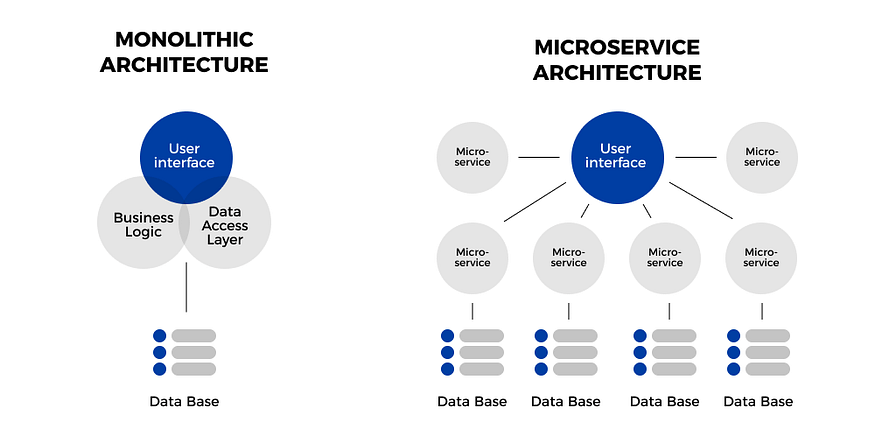
\includegraphics[scale=0.5]{Pictures/3_micro_mono.png}
    \caption{Monolithic and Microservices architectures\textsuperscript{\cite{monoliths_medium}}.}
    \label{fig:3_micro_mono}
\end{figure}

In Figure \ref{fig:3_micro_mono}, the distinction between a microservices approach and monolithic
architecture is illustrated. The latter is characterized by tightly coupled and interdependent
software components, any changes require building and deploying the entire stack, which can be slow
and error-prone. Microservices are designed to overcome these limitations by decomposing
functionality into separate services, each with a specific role, thus providing a more flexible and
scalable architecture. The table \ref{tab:micro_vs_mono} contains an overview of the differences
between the two approaches.

\begin{table}
    \centering
    \begin{tabular}{|l|p{5cm}|p{5cm}|}
        \hline
        \textbf{}            & \textbf{Monolithic}                                                                    & \textbf{Microservices}                                                       \\ \hline
        \textbf{Deployment}  & Simple and fast deployment of the entire system                                        & Requires distinct resources, making orchestrating the deployment complicated \\ \hline
        \textbf{Scalability} & It is hard to maintain and handle new changes; the whole system needs to be redeployed & Each element can be scaled independently without downtime                    \\ \hline
        \textbf{Agility}     & Not flexible and impossible to adopt new tech, languages, or frameworks                & Integrate with new technologies to solve business purposes                   \\ \hline
        \textbf{Resiliency}  & One bug or issue can affect the whole system                                           & A failure in one microservice does not affect other services                 \\ \hline
        \textbf{Testing}     & End-to-end testing                                                                     & Independent components need to be tested individually                        \\ \hline
        \textbf{Security}    & Communication within a single unit makes data processing secure                        & Interprocess communication requires API gateways raising security issues     \\ \hline
        \textbf{Development} & Impossible to distribute the team’s efforts due to the huge indivisible database       & A team of developers can work independently on each component                \\ \hline
    \end{tabular}
    \caption{Comparison of Monolithic and Microservices architectures\textsuperscript{\cite{monoliths_avenga}}.}
    \label{tab:micro_vs_mono}
\end{table}

\section{How to Model Microservices}
This section is dedicated to exploring key principles such as information hiding, coupling, and
cohesion, which are crucial in shaping our approach to defining the limits of our microservices. We
will place a particular focus on domain-driven design, a highly effective strategy that plays a
crucial role in establishing the boundaries of your microservices. This approach not only maximizes
their advantages but also effectively reduces potential risks.

\subsection{Boundaries}
Our goal is to design microservices that can be independently modified, deployed, and have their
features released to users without relying on others. The ability to update a single microservice
independently from the others is crucial. At their core, microservices represent a type of modular
decomposition, but with network interactions between modules. This means we can rely on a lot of
prior art in the space of modular software to assist in defining our boundaries. Bearing this in
mind, we will delve into three essential concepts crucial for identifying effective microservice
boundaries: information hiding, cohesion, and coupling\textsuperscript{\cite{microservices_book}}.

\subsubsection{Information Hiding}
Information hiding is a concept developed by David Parnas to look at the most effective way to
define module boundaries\textsuperscript{\cite{microservices_model_1}}. Information hiding aims to
conceal as much detail as possible within a microservice boundary. Parnas
write\textsuperscript{\cite{microservices_model_2}}:

\begin{quote}
    The connections between modules are the assumptions which the modules make about each other.
\end{quote}

Reducing assumptions between modules in microservices simplifies their connections, making it easier
to modify one module without affecting others. This approach also allows developers to make safer
changes, as they understand how their module is used by others, preventing the need for changes in
upstream components. Additionally, in microservices, such modifications can be deployed
independently, enhancing the benefits outlined by Parnas: faster development, better
comprehensibility, and increased flexibility.

% \begin{itemize}
%     \item \textbf{Improved development time}: Enabling independent development of modules
%           facilitates parallel work, thus diminishing the complexities often associated with increasing
%           the number of developers on a project.
%     \item \textbf{Comprehensibility}: The ability to examine and comprehend each module separately
%           simplifies the process of grasping the system’s overall functionality.
%     \item \textbf{Flexibility}: The independence of modules allows for alterations in one without
%           necessitating changes in others. Furthermore, this independence provides the flexibility to
%           recombine modules in various configurations, creating new functionalities.
% \end{itemize}

\subsubsection{Coupling and Cohesion}
The concepts of coupling and cohesion are integral to the structure and stability of microservice
architectures. Understanding their interplay helps in designing systems that are both stable and
efficient.
% Cohesion refers to how closely related the functionalities within a microservice are,
% aiming for a strong internal unity. Coupling, on the other hand, deals with the degree of
% interdependence between different microservices, where the goal is to minimize dependencies to
% achieve loose coupling. 
Achieving the right balance between these two aspects is crucial for the
effective functioning of microservices.

\begin{itemize}
    \item \textbf{Cohesion}: Cohesion in microservices is about strategically grouping related
          business functionalities to reduce the need for changes across multiple areas. It emphasizes
          consolidating similar behaviors in a single location, which streamlines the process of
          modification and deployment. This approach leads to strong cohesion, where closely related
          functionalities are contained within a single microservice, thereby enabling faster and more
          secure updates and changes.
    \item \textbf{Coupling}: Coupling in the context of microservices involves designing services in
          a way that changes in one do not require modifications in others. This design principle promotes
          minimal inter-service knowledge, thereby reducing dependencies between different services. The
          ideal state of loose coupling is achieved when services have minimal interactions with each
          other, maintaining their independence. This approach significantly reduces the risks associated
          with tightly interconnected systems, ensuring more robust and flexible service architecture.
\end{itemize}

This balance is not only about the technical aspects but also about making pragmatic decisions that
fit the specific context and challenges of the project.

\subsubsection{Types of Coupling}
The concept of coupling in system design is nuanced and not as straightforward as it might initially
appear. While it's true that excessive coupling can lead to various challenges in system
architecture, some level of coupling is inevitable and, in certain cases, necessary. The key
objective in effective system design is not to eliminate coupling entirely but to manage and
minimize its extent.

\begin{figure}
    \centering
    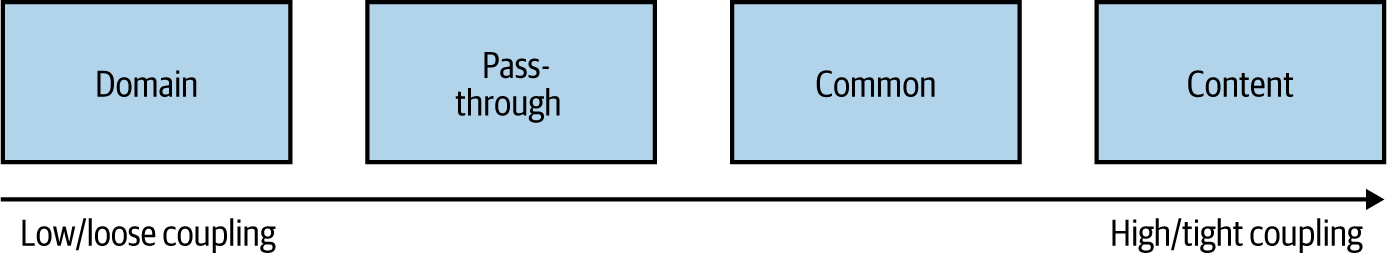
\includegraphics[scale=0.5]{Pictures/3_types_coupling.png}
    \caption{The different types of coupling, from loose (low) to tight (high)}.
    \label{fig:3_types_coupling}
\end{figure}

The different types of coupling\textsuperscript{\cite{microservices_book}}, as depicted in Figure
\ref{fig:3_types_coupling}, provide a comprehensive spectrum, ranging from low to high. Low coupling
is generally desirable as it indicates a system where components operate independently, enhancing
flexibility and ease of maintenance. High coupling, on the other hand, suggests a tightly
interlinked system where changes in one component can have significant ripple effects, making it
less desirable due to the increased complexity and risk involved. Understanding these variations and
their implications is crucial for designing robust, scalable, and maintainable systems.

\begin{itemize}
    \item \textbf{Domain Coupling}: Domain coupling refers to a scenario where one microservice
          depends on another for specific functionalities. While such interactions are largely inevitable
          in a microservice architecture, where collaboration among multiple services is essential for
          system operation, it's important to minimize these interactions. It is a form
          of loose coupling in microservices, but can lead to issues if a service relies too heavily on many
          downstream services, suggesting over-centralization of logic. Problems may also arise from
          exchanging complex data sets between services. It's advisable to share only essential
          information and minimize data exchange.
    \item \textbf{Pass-Through Coupling}: Pass-through coupling in microservices occurs when one
          microservice transmits data to another solely for the use of a subsequent downstream service.
          This form of coupling is particularly challenging within implementation strategies, as it
          suggests that the initiating service is aware not only of the direct recipient microservice but
          may also need to understand the functioning of the microservice further down the chain. This
          creates a complex interdependency where knowledge of multiple services and their interactions
          becomes necessary, complicating the architecture.
    \item \textbf{Common Coupling}: Common coupling in microservices refers to the scenario where
          multiple services utilize the same data set, such as a shared database, memory, or filesystem.
          This coupling becomes problematic when changes to the data's structure affect several services
          simultaneously. For example, if the schema of a commonly used database changes incompatibly, all
          services relying on it need updates. Additionally, common coupling can lead to resource
          contention issues, as multiple services accessing the same database or filesystem may strain or
          even incapacitate that resource. While sometimes manageable, common coupling often indicates a
          lack of cohesion in the system and can pose operational challenges, making it one of the less
          desirable forms of coupling.
    \item \textbf{Content Coupling}: Content coupling occurs when an upstream service intrusively
          modifies the internal state of a downstream service, commonly by directly accessing and altering
          the latter's database. This is subtly different from common coupling, where multiple services
          interact with a shared dataset, but acknowledge it as an external, uncontrollable dependency.
          Content coupling blurs ownership lines, complicating system modifications for developers. A
          clear distinction in microservices between changeable and unchangeable elements is crucial.
          Developers must be aware of the service contract exposed to external parties to avoid disrupting
          upstream consumers. While common coupling shares some issues with content coupling, the latter
          introduces additional complexities, often termed pathological coupling. Direct external access
          to a database challenges the definition of what can be safely altered and what cannot,
          undermining the principle of information hiding. Therefore, content coupling is best avoided due
          to these inherent complications.
\end{itemize}

% volendo puoi mettere le immagini

\subsection{Domain-Driven Design}
In defining microservice boundaries, we primarily focus on the domain itself, applying domain-driven
design (DDD) to model our domain more effectively. DDD, as introduced by Eric Evans in
"Domain-Driven Design"\textsuperscript{\cite{ddd_book}}, provides key concepts that are crucial in
this context. These include Ubiquitous Language, which ensures uniform language usage across the
domain; Aggregates, which group related domain objects into a single unit; and Bounded Context,
which sets the scope of applicability for a particular model. These principles play a vital role in
guiding our microservice architecture strategy.

\subsubsection{Ubiquitous Language}
Ubiquitous language emphasizes the importance of aligning the terminology in our code with the terms
used by the users. This commonality of language between the development team and the end users
simplifies modeling the real-world domain and enhances communication. Integrating real-world
language into the code streamlines the development process. It allows developers, when handling
tasks or stories, to quickly grasp the requirements and objectives, as these are expressed in terms
familiar to both the product owner and the development team.

\subsubsection{Aggregates}
Aggregates in microservice architecture are envisioned as self-contained units, each with its own
state, identity, and life cycle that mirrors real-world entities. These aggregates are apt for
implementation as state machines, given their inherent life cycles. The design focuses on
consolidating the code that manages state transitions with the aggregate's state itself. Typically,
a single microservice is responsible for one aggregate, but it may handle several. For instance, an
Invoice aggregate would include various line payments, each significant only within the context of
the overall Invoice aggregate.
\newline\newline
A microservice's role extends to managing the life cycle and data storage of one or several types of
aggregates. Should a different service need to modify an aggregate, it must either directly request
this change or prompt the aggregate to initiate its own state transitions, possibly in response to
events from other microservices. Aggregates are designed with the capability to reject inappropriate
state transition requests, underscoring the importance of preventing illegal state changes in their
implementation.

\subsubsection{Bounded Context}
A bounded context usually reflects a larger section of an organization, with clear responsibilities
within its boundaries. This concept focuses on concealing the finer details of implementation,
safeguarding internal aspects that aren't necessary for external understanding or involvement.
\newline\newline
In terms of structure, a bounded context comprises one or more aggregates. While some of these
aggregates might be visible externally, others remain internal to maintain the integrity of the
context. Bounded contexts can also form relationships with other contexts, translating into
dependencies between services in a microservice architecture.
\newline\newline
For instance, a warehouse service can be seen as a bounded context, bustling with activities like
processing outgoing orders, receiving new inventory, and other logistical tasks. In a different
bounded context, such as the finance department, the focus shifts to less dynamic but equally vital
functions like managing payroll and handling financial transactions. Each context operates within
its own realm of responsibilities but may interact with or depend on other contexts, reflecting the
interconnected nature of services in a microservices setup.

\subsubsection{Domain-Driven Design in Microservices}
Domain-Driven Design (DDD) is effective in microservices architecture due to its focus on bounded
contexts which conceal internal complexities and present clear boundaries to the system. These
contexts aid in maintaining stable microservice boundaries by ensuring that internal changes do not
affect other system parts. When systems are segmented along bounded contexts, modifications for
business needs are confined to specific microservices, streamlining deployment and reducing the
complexity of changes.

\newpage

\begin{figure}
    \centering
    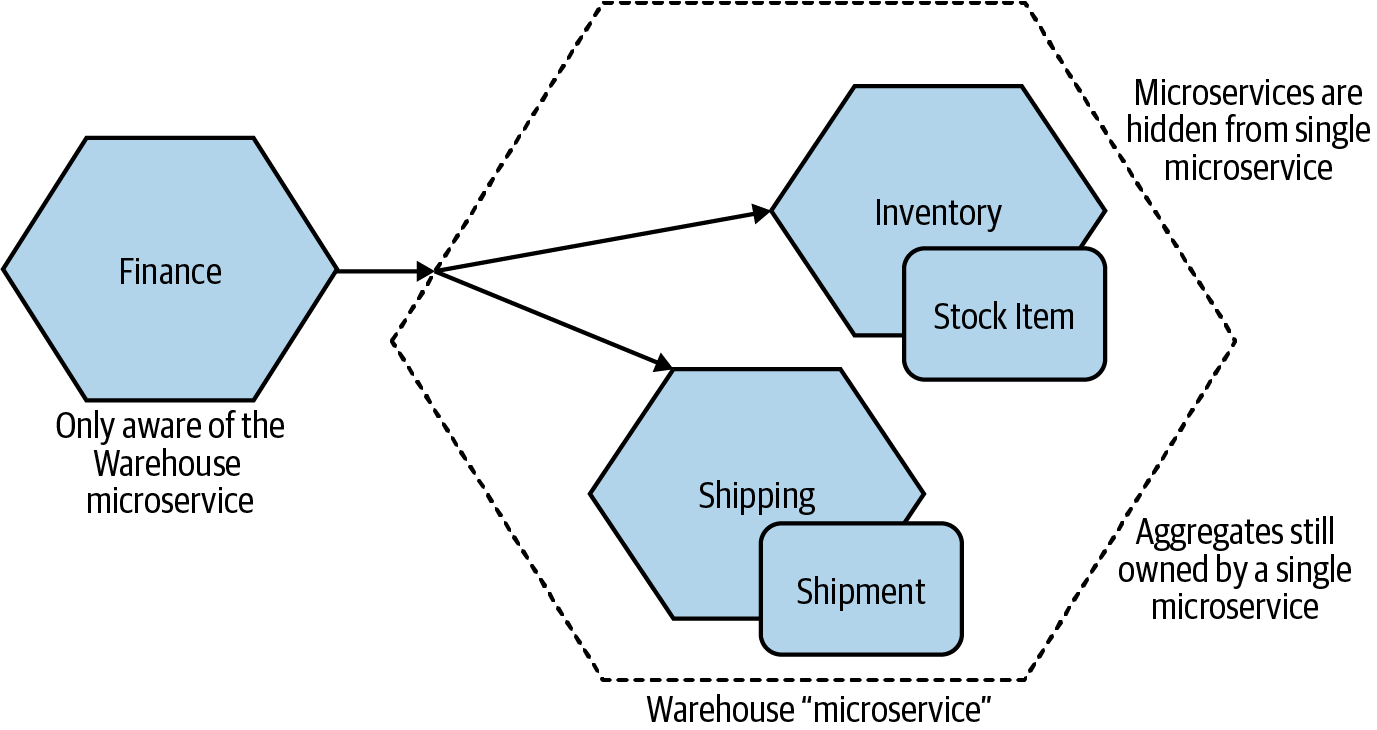
\includegraphics[scale=0.5]{Pictures/3_ddd.png}
    \caption{The Warehouse service internally has been split into Inventory and Shipping microservices}.
    \label{fig:3_ddd}
\end{figure}

Aggregates and bounded contexts both provide cohesive units with clear interfaces to the larger
system. Aggregates are focused state machines for single domain concepts, while bounded contexts
group these aggregates and represent them to the outside world. These constructs are ideal for
defining microservice boundaries. Initially, it's beneficial to work with services that cover
complete bounded contexts. If needed, services can later be divided into smaller ones without
splitting individual aggregates, keeping such internal decisions invisible to external stakeholders.
For instance, a Warehouse service may internally be divided into Inventory and Shipping, but
externally it remains a singular Warehouse microservice to users, as depicted in the figure
\ref{fig:3_ddd}.

\subsection{Event-Driven Architecture}
Event-Driven Architecture (EDA) is a software design paradigm that facilitates communication between
services or components through the asynchronous exchange of events. It is essential in microservices
for enabling decoupling, scalability, and reactive programming. This architecture allows real-time
information flow between applications, microservices, and connected devices as events occur,
promoting what is known as loose coupling. In EDA, applications and devices communicate without
needing to know the specific sources or destinations of the information, maintaining isolated
services with single responsibilities within a system\textsuperscript{\cite{event_1}}.

\subsubsection{Example Architecture}
The image \ref{fig:3_event_example} depicts an event-driven architecture for an e-commerce
site, showcasing how different components interact via events to enable a responsive and resilient
system. Event Producers like a retail website, mobile app, and point-of-sale system generate events
such as new orders or stock queries. These events are routed by the Event Router, which ingests,
filters, and directs them to the appropriate Event Consumers. The consumers, such as the Warehouse
Management Database, Finance System, and Customer Relations, act upon these events to update
inventory, financial records, and customer service actions, respectively. This architecture ensures
the site remains operational and efficient, even during high traffic, by reacting to real-time data
without overloading the system.

\begin{figure}
    \centering
    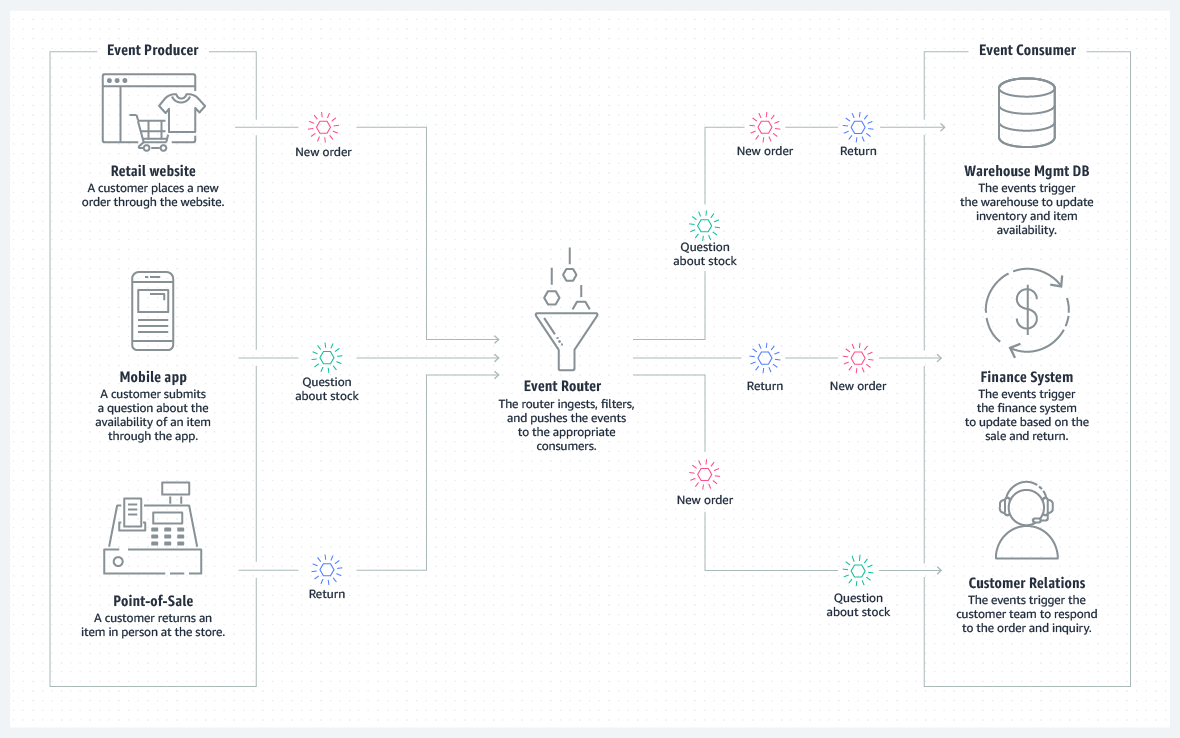
\includegraphics[scale=0.35]{Pictures/3_event_example.png}
    \caption{Example of an event-driven architecture\textsuperscript{\cite{event_2}}.}
    \label{fig:3_event_example}
\end{figure}

\newpage

\subsubsection{How it works}

\begin{figure}
    \centering
    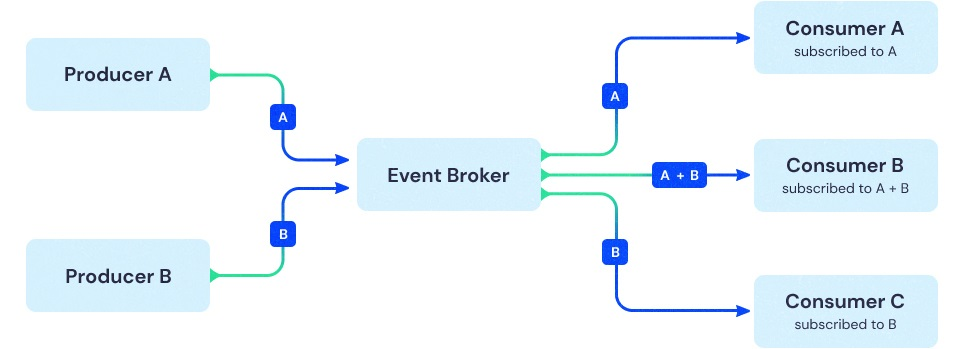
\includegraphics[scale=0.6]{Pictures/3_event_works.jpg}
    \caption{How event-driven architecture works\textsuperscript{\cite{event_4}}.}
    \label{fig:3_event_works}
\end{figure}

In this architecture pattern, events are generated by producers and captured by an event bus,
which routes them to the appropriate consumer services that process the event and may generate new
events. This model enables decoupled and asynchronous interactions, allowing microservices to
operate independently while responding to changes and inputs. EDA is scalable and allows for
immediate response to events, with no need for point-to-point integrations, making it easy to add
new consumers to the system\textsuperscript{\cite{event_3}}.

\begin{table}
    \centering
    \begin{tabular}{|l|p{0.6\linewidth}|}
        \hline
        \textbf{Component}      & \textbf{Description}                                                    \\ \hline
        \textbf{Event}          & The core of EDA, an event is a significant change in state, which other
        parts of the application can listen to and react upon.                                            \\ \hline
        \textbf{Event Producer} & A component that generates events.                                      \\ \hline
        \textbf{Event Consumer} & A component that processes events.                                      \\ \hline
        \textbf{Event Bus}      & A channel through which events are routed from producers to the
        appropriate consumers.                                                                            \\ \hline
    \end{tabular}
    \caption{Event-driven architecture components\textsuperscript{\cite{event_3}}.}
    \label{tab:eda_components}
\end{table}

\subsubsection{Models}
The table \ref{tab:eda_models} summarizing the different models of Event-Driven Architecture
along with their descriptions and examples\textsuperscript{\cite{event_5}}:

\newpage

\begin{table}
    \centering
    \begin{tabular}{|p{0.2\linewidth}|p{0.5\linewidth}|p{0.2\linewidth}|}
        \hline
        \textbf{Model}                    & \textbf{Description}                                                                                                                    & \textbf{Example}   \\ \hline
        \textbf{Process Manager}          & The orchestrator that manages a workflow or process, performing business logic and triggering events to other consumers.                & AWS Step Functions \\ \hline
        \textbf{Event Sourcing}           & Stores events to calculate state, with downstream projections using this to calculate their view of the world. It's great for auditing. & Amazon DynamoDB    \\ \hline
        \textbf{Event Streaming}          & Used for real-time information processing, such as user interactions. Messages are placed onto a stream for consumers to process.       & Amazon Kinesis     \\ \hline
        \textbf{Point-to-Point Messaging} & Sends messages to a channel for downstream consumers to process, allowing for concurrent processing and scalability.                    & Amazon SQS         \\ \hline
        \textbf{Change Data Capture}      & Reacts to changes made against data, with consumers attached to these changes for processing.                                           & Amazon DynamoDB    \\ \hline
        \textbf{Pub/Sub}                  & Fires notifications out to downstream consumers, fanning out events and allowing consumers to get their own copy of the event.          & Amazon EventBridge \\ \hline
    \end{tabular}
    \caption{Models of Event-Driven Architecture.}
    \label{tab:eda_models}
\end{table}

\subsubsection{Advantages}
Event-Driven Architecture offers several compelling advantages when applied to microservices. One of
its primary benefits is loose coupling, which allows services to operate independently, thereby
reducing dependencies and simplifying maintenance. This loose coupling also contributes to the
scalability of the system; services can be scaled up or down independently, and new consumers can be
integrated without significant disruption to the existing ecosystem. Moreover, EDA provides
flexibility and dynamism, enabling the system to quickly adapt to new business requirements by
simply adding new event consumers. Finally, from a cost perspective, EDA systems are inherently
efficient since they are push-based rather than pull-based, eliminating the need for continuous
polling to check for events, which can lead to significant cost savings on compute and network
resources\textsuperscript{\cite{event_6}}\textsuperscript{\cite{event_2}}.

\subsubsection{Disadvantages}
While Event-Driven Architecture presents numerous benefits for microservices, it also introduces a
set of challenges. The inherent complexity of designing and managing an event-driven system is
non-trivial, often requiring a sophisticated understanding of distributed systems. Testing,
debugging and monitoring in a highly distributed systems adds another layer of complexity,
necessitating robust and comprehensive strategies for tracing and logging. Performance can be
impacted as well, given that the event broker or bus acting as a middle man between producers and
consumers might introduce latency, potentially leading to longer execution times for event
processing. Finally, the principle of eventual consistency in EDA means that services might process
and react to the same event at different times, which can complicate transactional integrity and
require careful handling to maintain system accuracy and
reliability\textsuperscript{\cite{event_6}}\textsuperscript{\cite{event_3}}.

\subsection{Workflow Management}
In the environment of microservices, the complexity of interactions extends beyond the simple
communication between two services. A critical aspect is the orchestration of multiple microservices
working together to execute comprehensive business processes. This orchestration requires a nuanced
approach to maintain the system's integrity and efficiency.
\newline\newline
In this section, we'll explore how microservices can collaborate on workflows and processes. We'll
delve into strategies like distributed transactions, which attempt to address these coordination
challenges, and examine the saga pattern, an advanced concept that provides a structured approach to
manage long-running, distributed business transactions within microservice architectures.

\subsubsection{Database Transactions}
In computing, transactions are a series of actions completed as a single unit, ensuring all changes
are made or none if an error occurs. This concept is crucial in databases, where transactions (like
insertions, deletions, or updates) must be successful, often spanning multiple tables. The term
database transactions usually refers to ACID transactions\textsuperscript{\cite{microservice_acid}},
which is explained in table \ref{tab:acid}.

\begin{table}
    \centering
    \begin{tabular}{|c|l|p{0.6\linewidth}|}
        \hline
        \textbf{Letter} & \textbf{Stands for} & \textbf{Description}                                                                             \\ \hline
        A               & Atomicity           & Ensures that all parts of a transaction are completed successfully, or none at all.              \\ \hline
        C               & Consistency         & Guarantees that a transaction only brings the system from one valid state to another.            \\ \hline
        I               & Isolation           & Ensures that transactions are performed independently and transparently.                         \\ \hline
        D               & Durability          & Assures that once a transaction is committed, it will remain so, even in the event of a failure. \\ \hline
    \end{tabular}
    \caption{ACID properties of database transactions}
    \label{tab:acid}
\end{table}

In microservices, ACID transactions apply to local operations within a single microservice,
complicating atomic operations across multiple services. Unlike a monolithic database that ensures
atomicity through ACID properties, a distributed microservices system handles changes across
separate databases, as depicted in Figure \ref{fig:3_transaction}. This leads to independent
transactions that may succeed or fail separately, lacking atomicity for the entire operation.

% When it comes to microservices, the use of ACID transactions still applies, but their scope is
% confined to the local operations within an individual microservice. This presents a challenge, as
% the atomicity of operations across multiple microservices is not inherently guaranteed. For
% instance, an operation that changes a customer's status and removes them from a "PendingEnrollments"
% table is straightforward in a monolithic single database environment due to the ACID properties.
% However, as shown in Figure \ref{fig:3_transaction}, in a distributed microservices setup these
% changes are split across different databases and hence become two distinct transactions. This
% separation means that we may no longer have the atomicity of the entire operation, as each
% transaction may succeed or fail independently.

\begin{figure}
    \centering
    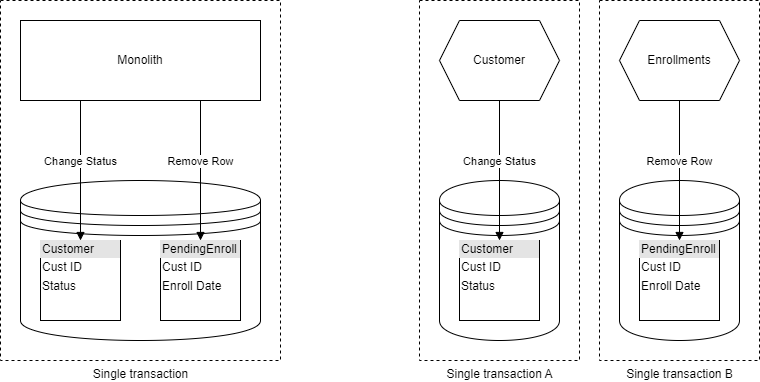
\includegraphics[scale=0.5]{Pictures/3_transaction.png}
    \caption{Example that show the difference between monolithic and microservices transactions.}
    \label{fig:3_transaction}
\end{figure}

\subsubsection{Distributed transaction - Two-Phase Commit}
The Two-Phase Commit (2PC) algorithm facilitates transactional updates across distributed systems,
ensuring atomic transaction commits across multiple nodes. Essentially, it mandates that all
involved nodes must either commit or abort together, maintaining the principle of atomic
transactions\textsuperscript{\cite{2pc_1}}. Unfortunately, 2PC is often viewed as impractical for
microservice architectures\textsuperscript{\cite{microservices_book}}, thus this section explores the
reasons behind this perspective, analyzing the limitations and challenges of applying 2PC in such
contexts.
\newline\newline
In the figure \ref{fig:3_2pc} we can see an example of the 2PC protocol process. The protocol is
divided into two phases: the prepare phase and the commit phase. Initially, in the prepare phase,
microservices are prompted to ready themselves for a potential atomic data change. Following this,
the commit phase involves directing these microservices to execute the actual changes. Central to
this process is a global coordinator, responsible for overseeing the transaction's lifecycle and
engaging with microservices during both the prepare and commit phases. This coordinator is pivotal
in determining whether the nodes can commit the proposed transaction and in issuing the final
command to commit or abort\textsuperscript{\cite{2pc_1}}\textsuperscript{\cite{2pc_2}}.

\newpage

\begin{figure}
    \centering
    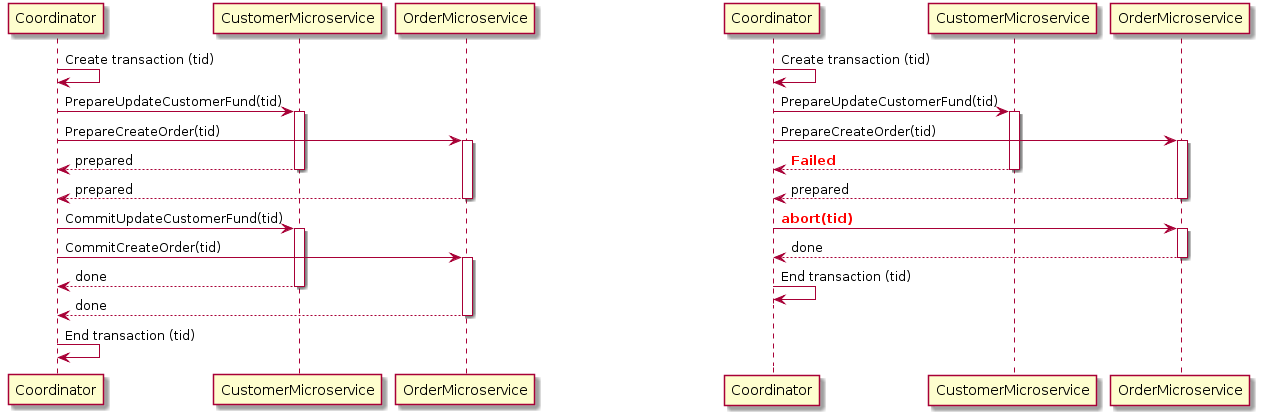
\includegraphics[scale=0.55]{Pictures/3_2pc.png}
    \caption{Example of the 2PC protocol process\textsuperscript{\cite{2pc_2}}.}
    \label{fig:3_2pc}
\end{figure}

The major benefit of 2PC protocol is that it is a robust mechanism for ensuring consistency across
distributed systems. Its dual phases — prepare and commit — assure that transactions are atomic,
making all microservices commit successfully or none at all, preventing partial updates.
Additionally, 2PC enforces read-write isolation, ensuring that any modifications remain invisible
until the coordinating node finalizes the commit, maintaining transaction integrity throughout the
process\textsuperscript{\cite{2pc_2}}.
\newline\newline
Although 2PC ensures atomicity, its limitations make it less suitable for numerous
microservice-based systems\textsuperscript{\cite{2pc_2}}. The main issue of 2pc protocol
are\textsuperscript{\cite{2pc_3}}:

\begin{itemize}
    \item \textbf{Blocking}: The protocol locks objects until a transaction is complete, causing
          potential delays and deadlock.
    \item \textbf{Latency}: Waiting for all participant responses before proceeding adds to the
          transaction time.
    \item \textbf{Coordinator Risk}: The Transaction Coordinator is a critical point that can fail,
          blocking all transactions.
    \item \textbf{Participant Performance}: The entire transaction's speed is tied to the slowest
          participant, with failures necessitating full rollbacks.
\end{itemize}

\subsubsection{Saga distributed transactions pattern}
As described so far, to avoid coupling between microservices, the database-per-microservice pattern
is utilized, allowing each service to manage its own data. This method offers several advantages:
select the most suitable data store type, scale it independently, and maintain isolation from
failures in other services\textsuperscript{\cite{ms_sagas}}. This pattern has a drawback: it does
not support ACID transactions across multiple services. To overcome this limitation, the Saga
pattern can be employed.
\newline\newline
Unlike a two-phase commit, the saga pattern is designed to effectively coordinate multiple state
changes, ensuring data consistency and avoiding resource locks across microservices. It accomplishes
this by decomposing the process into separate, independently executable activities. The adoption of
the saga pattern necessitates the explicit modeling of business processes, which can yield
significant benefits\textsuperscript{\cite{microservices_book}}.

\begin{figure}
    \centering
    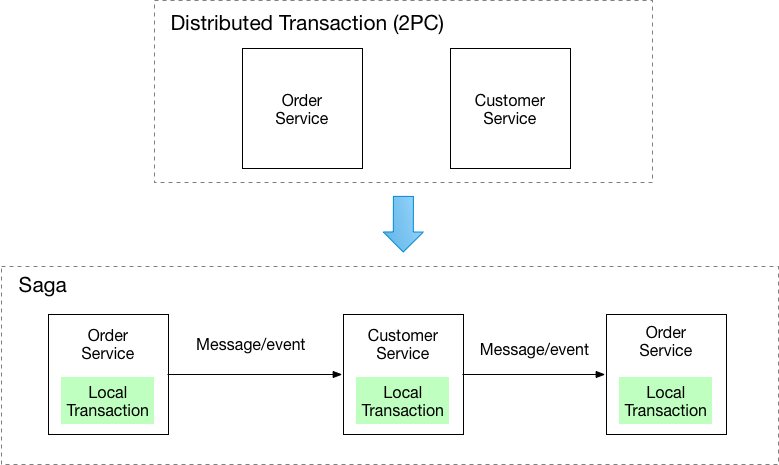
\includegraphics[scale=0.5]{Pictures/3_saga.png}
    \caption{From 2pc to Saga pattern\textsuperscript{\cite{io_sagas}}.}
    \label{fig:3_saga}
\end{figure}

How showed in figure \ref{fig:3_saga}, the Saga pattern manages transactions across multiple
services through a sequence of local transactions, each serving as an atomic work effort by a saga
participant. In this pattern, every local transaction updates the database and publishes a message
or event to initiate the subsequent local transaction within the saga. If any local transaction
fails, typically due to a violation of business rules, the saga responds by executing compensating
transactions to reverse the changes made by earlier local transactions. This approach ensures
consistent and reliable transaction management in complex, distributed
systems\textsuperscript{\cite{ms_sagas}}\textsuperscript{\cite{io_sagas}}.
\newline\newline
The key benefit of Saga is maintaining data consistency across multiple services without needing
distributed transactions. However, it introduces complexities: developers must create compensating
transactions to reverse earlier changes, and debugging becomes challenging, especially as the number
of services involved increases.
When a client initiates a saga through a synchronous request (like an HTTP POST), determining the
saga's outcome is crucial. This can be managed in several ways\textsuperscript{\cite{io_sagas}}:

\begin{itemize}
    \item \textbf{Immediate Response Post-Completion}: The service responds after the saga
          completes, ensuring a definitive outcome but possibly causing delays.
    \item \textbf{Initiation Acknowledgement with Periodic Polling}: The service acknowledges the
          saga's start, and the client periodically checks for the outcome.
    \item \textbf{Initiation Acknowledgement with Event Notification}: The service sends an initial
          response and notifies the client via an event (e.g., websocket) upon saga completion.
\end{itemize}

There are two prevalent methods for implementing the Saga pattern: choreography and orchestration.
Each method presents unique challenges and requires specific technologies to effectively coordinate
the workflow.

\subsubsection{Choreography-based saga}
Choreography in sagas refers to a decentralized method of coordination where participants
communicate through the exchange of events, without relying on a central control point. In this
approach, each local transaction emits domain events that activate local transactions in
other services\textsuperscript{\cite{ms_sagas}}.

\begin{figure}
    \centering
    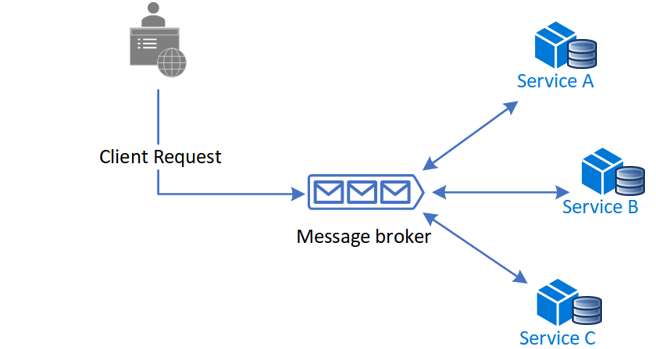
\includegraphics[scale=0.55]{Pictures/3_choreography.png}
    \caption{Choreography-based saga\textsuperscript{\cite{ms_sagas}}.}
    \label{fig:3_choreography}
\end{figure}

The workflow is well-suited for simpler processes with fewer participants, as it does not
necessitate complex coordination logic or the implementation and maintenance of an additional
service. This decentralization also prevents the emergence of a single point of failure. However,
the approach has its limitations; as the workflow grows, it becomes increasingly challenging to
track the interactions and commands between saga participants, potentially leading to cyclic
dependencies. Integration testing can be complicated, requiring all services to be
active to effectively simulate a transaction, posing a considerable challenge in practical
applications\textsuperscript{\cite{ms_sagas}}.

\subsubsection{Orchestration-based saga}
Orchestration in sagas involves a central controller directing saga participants on which local
transactions to carry out. The orchestrator manages all transactions, instructing participants on
specific operations in response to events. It is responsible for executing saga requests,
maintaining and interpreting the state of each task, and managing failure recovery through
compensating transactions\textsuperscript{\cite{ms_sagas}}.

\begin{figure}
    \centering
    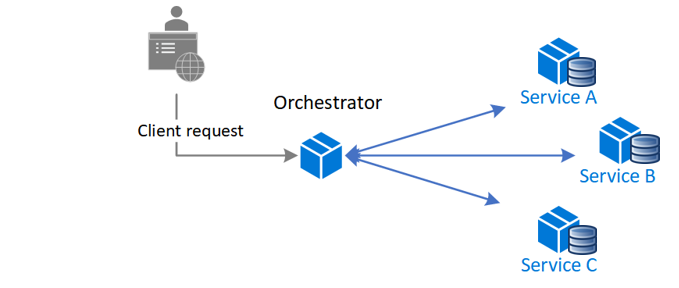
\includegraphics[scale=0.55]{Pictures/3_orchestrator.png}
    \caption{Orchestration-based saga\textsuperscript{\cite{ms_sagas}}.}
    \label{fig:3_orchestration}
\end{figure}

This pattern is advantageous for complex workflows with numerous participants or when incorporating
new participants over time, as it allows complete control over each participant and their
activities. This approach eliminates cyclical dependencies by having the orchestrator solely depend
on the saga participants and simplifies business logic by clearly separating concerns. Anyway, it
introduces additional design complexities by requiring the implementation of specific coordination
logic, and the orchestrator itself becomes a potential point of failure, managing the entire
workflow and thus presenting a risk to the system's stability\textsuperscript{\cite{ms_sagas}}.

\section{Serverless}
\subsection{Introduction}
The advent of serverless computing marks a significant shift in the way applications are developed
and managed, especially within the domain of microservices. As the architecture of an application
expands, operational responsibilities grow correspondingly. Public cloud providers have risen to
this challenge by offering an extensive suite of managed services, ranging from managed database
instances and Kubernetes clusters to message brokers and distributed file systems. Leveraging these
managed services translates to offloading substantial operational workload to third-party experts,
who are often more equipped to manage these complex tasks\textsuperscript{\cite{microservices_book}}.
\newline\newline
Within the serverless offerings, services that facilitate Event-Driven Architecture hold a
place of prominence. Serverless platforms inherently support EDA by abstracting away the
infrastructure, allowing developers to concentrate on code and event flows rather than server
management. Products such as message brokers, storage solutions, and databases are designed to
seamlessly integrate with event-driven models, providing a responsive and efficient means to trigger
and scale microservices based on real-time events\textsuperscript{\cite{event_book}}.
\newline\newline
Function as a Service (FaaS), a cornerstone of serverless offerings, perfectly complements EDA by
providing a mechanism to deploy code that automatically responds to events without the need for
explicit server provisioning. Developers simply deploy their functions, which are then executed in
response to events, scaling automatically with the volume of requests. This serverless, event-driven
model significantly reduces the complexity of scaling and managing infrastructure, allowing
developers to focus on building responsive, efficient, and modern cloud-native
applications.\textsuperscript{\cite{microservices_book}}.

\subsubsection{Example of Serverless}

\begin{figure}
    \centering
    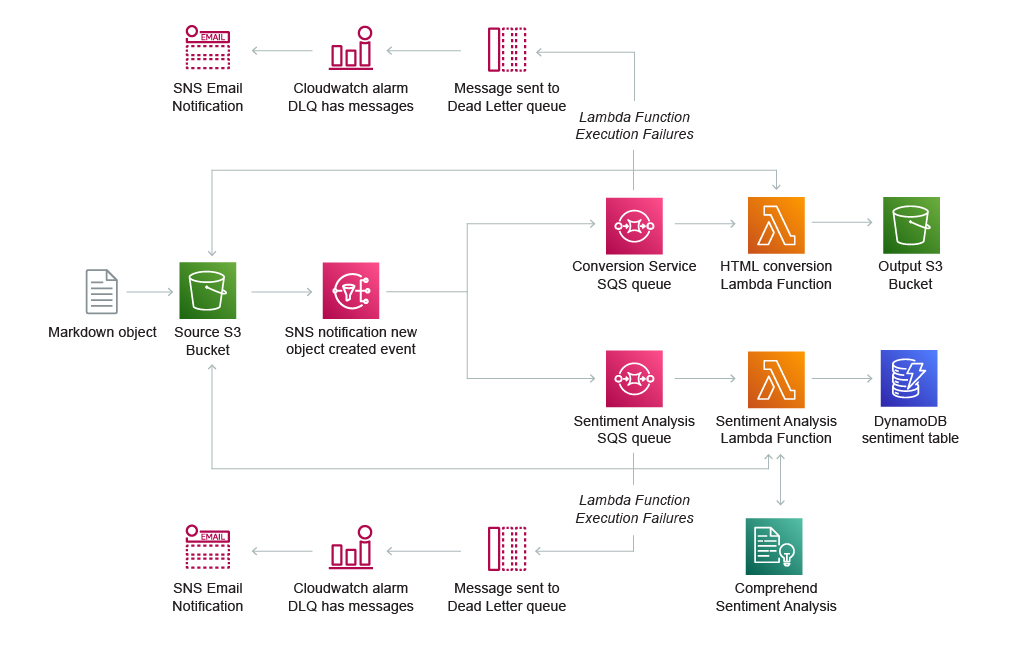
\includegraphics[scale=0.4]{Pictures/3_serverless_example_2.jpg}
    \caption{Example of Serverless Architecture.}
    \label{fig:3_serverless_example}
\end{figure}

The diagram \ref{fig:3_serverless_example} presents a serverless data processing architecture that
enables automatic handling of interview notes. When documents in Markdown format are uploaded to a
cloud-based storage service, the system is designed to trigger multiple automated workflows. The
first workflow involves a function-as-a-service platform, which is activated to convert the Markdown
documents into HTML files; these are then saved back to the storage service in a different location
for future access. Simultaneously, a second workflow commences, where another function is triggered
through a message queuing service to perform sentiment analysis on the text. The results of this
analysis are stored in a NoSQL database, allowing for efficient retrieval and analysis of the
processed data.

The entire process is monitored by a cloud-based monitoring system that watches over the message
queues and function executions. In case of any errors or malfunctions, an alert system is activated
to send notifications, ensuring that any issues are addressed promptly. This serverless architecture
exemplifies the modern approach to cloud computing, emphasizing automated, event-driven processes
that facilitate quick, scalable, and efficient data processing without the need for managing server
infrastructure\textsuperscript{\cite{serverless_1}}.

\subsection{Benefits}

\subsubsection{Cost-effective}
Serverless computing provides a cost-efficient model by charging only for the backend services when
code is executed, following an event-based model. This stands in contrast to traditional hosting
models, where costs are incurred for dedicated servers regardless of whether they are in active use.
By eliminating the need to provision, manage, and maintain physical servers, serverless computing
allows for significant cost savings. It is particularly economical for applications that do not run
continuously, as you pay solely for the resources utilized during the execution time, without the
overhead of server maintenance and
upgrades\textsuperscript{\cite{serverless_2}}\textsuperscript{\cite{serverless_3}}. However, it is
worth noting that for applications with constant runtime, serverless computing may not always be the
most cost-effective option\textsuperscript{\cite{serverless_4}}.

\subsubsection{Scalability}
Seamless scalability is a hallmark of serverless computing, allowing applications to adapt quickly
to fluctuating demands without the need for server management. It operates much like a bus system
that adjusts its capacity according to the number of passengers; serverless infrastructure
automatically scales up or down as user demand changes. This model ensures that server capacity is
precisely aligned with the necessary demand, providing ample resources when the number of user
requests increases without being constrained by the limitations of server storage and performance
capabilities\textsuperscript{\cite{serverless_2}}. This adaptability is considered one of the
primary benefits of serverless computing, enabling businesses, especially small and medium
enterprises (SMEs), to handle traffic surges efficiently and cost-effectively, ensuring service
continuity and performance without the disruptions commonly associated with traditional hosting
models\textsuperscript{\cite{serverless_3}}.

\subsubsection{Reliability}
Serverless computing inherently enhances application reliability due to multiple layers of built-in
redundancy. Since serverless applications are not tethered to a single origin server, they have the
flexibility to execute code from various locations, optimizing the function execution closer to the
end-user\textsuperscript{\cite{serverless_2}}\textsuperscript{\cite{serverless_3}}. This distributed
nature not only helps in reducing latency, thereby improving performance, but also contributes to
high availability. The risk of service outages or failures is significantly reduced, ensuring that
end-users have consistent and reliable access to the application
functions\textsuperscript{\cite{serverless_4}}.

\subsubsection{Increased productivity}
Serverless computing streamlines the development process, making it much faster and more efficient
to build and deploy applications. Developers are freed from the time-consuming tasks of server setup
and infrastructure maintenance, allowing them to concentrate on innovation and creativity without
being hindered by server constraints. As a result, developers can launch products more swiftly, as
there is no need for traditional server-side installations or workflow monitoring. The serverless
model enables direct code uploads and immediate function execution on the cloud provider’s
infrastructure. This agility extends to application updates and patches, which can be implemented
incrementally, targeting individual functions rather than disrupting the entire service. This
approach not only enhances development velocity but also reduces the resources allocated to DevOps,
leading to cost savings and allowing developers to focus purely on coding and product
improvement\textsuperscript{\cite{serverless_2}}\textsuperscript{\cite{serverless_3}}.

\subsubsection{Resource Utilisation}
The efficiency of serverless computing in terms of resource utilization marks a substantial
advancement towards greener technology practices. By engaging resources solely during code
execution, serverless platforms significantly minimize waste and avoid the energy costs associated
with powering idle servers. This responsiveness to real demand underscores serverless computing as
an eco-friendly choice, particularly appealing to organizations aiming to reduce their environmental
impact and achieve sustainability goals. Such a model is not only in line with ecological
considerations but also optimizes operational expenditures, positioning serverless computing as a
judicious approach for backend operations that are both environmentally and economically
conscious\textsuperscript{\cite{serverless_5}}.

\subsection{Drawbacks}
\subsubsection{Performance Issues}
Serverless architectures can encounter performance hiccups, particularly when reactivating idle
applications. Known as "cold start" latency, this issue arises when the serverless platform takes
additional time to provision resources for an application that hasn't been used recently. While
steps such as reducing code length can mitigate the impact, they may lead to a trade-off where
developers must manage a larger number of smaller, more manageable functions. Despite these efforts,
the initial delay in resource setup inherent to cold starts can still lead to slower response times
when an application is invoked after being dormant\textsuperscript{\cite{serverless_3}}.

\subsubsection{Limited Control}
In serverless computing, the cloud provider's management of the infrastructure results in developers
having limited control over the environment and certain application parameters. This lack of direct
control can hinder customization efforts and may pose issues if specific needs arise that require
adjustments at the infrastructure level. Additionally, cloud providers may offer limited support for
certain programming languages and runtime environments, which can restrict the technology stack
options for development\textsuperscript{\cite{serverless_2}}. Another consideration is the potential
for vendor lock-in; reliance on a single provider's serverless architecture can create dependencies
that complicate migrating to a different provider's services\textsuperscript{\cite{serverless_4}}.
These factors highlight the trade-offs between the convenience of serverless models and the need for
flexibility in application deployment and management.

\subsubsection{Increased Complexity}
While developers benefit from the reduced need to manage servers and scalability concerns, they are
faced with the intricacies of serverless architectures, such as state management, integration with
other services, and the unique security considerations these environments entail. Moreover, the
serverless paradigm often requires a different approach to application design, with a focus on
individual functions and services, which can be a departure from traditional monolithic
architectures. These elements can sometimes increase the cognitive load on developers and complicate
the application lifecycle management, especially for those accustomed to more control over the
server environment\textsuperscript{\cite{serverless_2}}\textsuperscript{\cite{serverless_3}}.

\subsubsection{Testing \& Debugging}
The abstraction inherent in serverless computing can obscure backend processes, complicating tasks
such as testing and debugging. Without traditional backend visibility, developers might find it
difficult to conduct in-depth inspections, detect faults, and identify errors within the cloud
environment, adopting more comprehensive strategies to anticipate and address potential issues. This
added complexity in monitoring and diagnosing problems requires a proactive approach to fault
prediction and management to minimize service disruptions for
users\textsuperscript{\cite{serverless_3}}. Debugging, in particular, presents a challenge as the
infrastructure's concealed nature takes away some of the direct troubleshooting tools that
developers rely on in more conventional setups\textsuperscript{\cite{serverless_4}}.

\subsubsection{Security concerns}
In serverless computing, the responsibility for security configurations largely rests with the cloud
provider, which can lead to concerns over limited control and potential security risks if the
provider's measures are not up to par. Careful evaluation of a provider's security protocols is
crucial, and applications must be designed with security best practices in mind to mitigate risks.
Despite the robust security measures typically employed by service providers, some users may still
be apprehensive about relinquishing direct control over security. Serverless architecture often
involves sharing resources between different clients on the provider's infrastructure, which
introduces the need for strong isolation policies to ensure that one client's activities do not
compromise another's security. Complying with these security considerations requires trust in the
provider's ability to safeguard the environment while also necessitating that developers stay
vigilant and informed about the security posture of their serverless
applications\textsuperscript{\cite{serverless_3}}\textsuperscript{\cite{serverless_4}}.

\subsection{Function-as-a-Service}
Functions-as-a-Service (FaaS) represents a modern "serverless" approach that has gained widespread
popularity for its ability to simplify the development and operation of applications. In FaaS,
functions - pieces of code - are executed in response to specific triggers, running only until their
task is completed. This model allows for efficient scaling, as the number of function executions
automatically adjusts based on the load, making it highly effective for event-driven systems where
workload can be unpredictable.\newline\newline
FaaS operates on a consumer/producer basis, where functions are transient, ceasing to exist after a
set duration along with their connections and state. This design necessitates careful planning in
function development but offers significant benefits. The cost efficiency is notable, as you incur
charges only for the time your code is running. Additionally, the FaaS platform manages the
operational complexities, such as automatically handling the spinning up and down of functions and
ensuring high availability and robustness with minimal effort from the developer.\newline\newline
The integration of FaaS in application development reduces operational overhead substantially,
making it an ideal choice for implementing simple to moderately complex solutions within
event-driven architectures. This approach allows developers to focus more on building functionality
without the burden of managing infrastructure, leading to more agile and responsive application
development\textsuperscript{\cite{event_book}}.

\begin{figure}
    \centering
    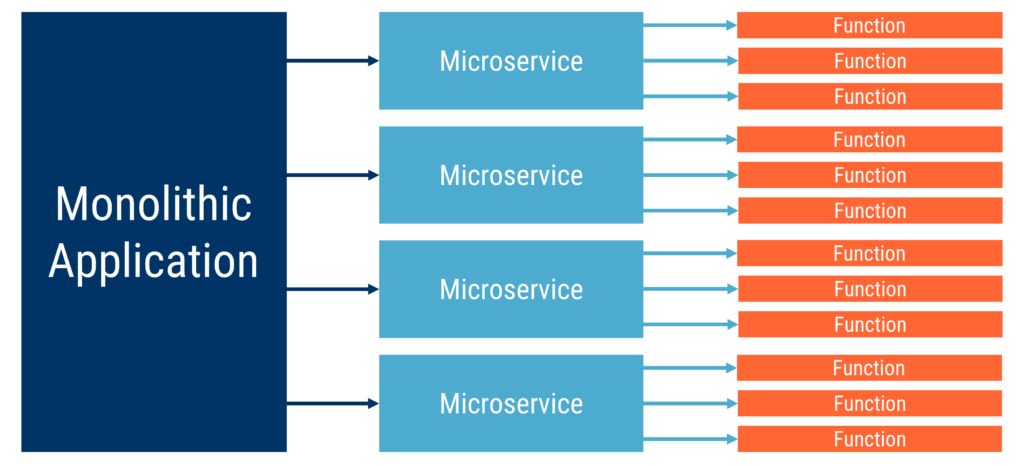
\includegraphics[scale=0.5]{Pictures/3_faas.png}
    \caption{Evolution of architectures\textsuperscript{\cite{serverless_9}}.}
    \label{fig:3_faas}
\end{figure}

\subsubsection{Cold Start and Warm Starts}
A "cold start" refers to the initial phase of a function in a FaaS (Function-as-a-Service)
environment when it is first activated or after a period of dormancy. During this phase, the system
initiates a container, loads the code, establishes connections with the event broker, and sets up
other necessary external resource connections. Once these preparatory steps are complete, the
function transitions to a "warm state," primed to process events. In this state, the function
actively processes events until it either completes its task or reaches a timeout, at which point it
enters a suspended or hibernation mode.\newline\newline
FaaS frameworks typically strive to optimize resource usage by reactivating these suspended
functions for subsequent tasks. In scenarios where there is a consistent flow of events, a function
may cycle between active processing and brief termination due to timeout. However, if the
connections to the event broker and state stores remain active during these short periods of
inactivity, the system can quickly resume processing with the reactivated function instance. This
reuse of function instances enhances efficiency, reducing the overhead and latency associated with
initializing a function from a cold start\textsuperscript{\cite{event_book}}.

\subsubsection{Maintaining State}
FaaS (Function-as-a-Service) platforms are designed for stateless operations, primarily due to the
ephemeral nature of functions. Since these functions have a limited lifespan, any FaaS-based
solution that requires statefulness typically relies on external stateful services. This design
choice aligns with the objective of FaaS providers to offer rapid, highly scalable processing
resources that are not constrained by the location of data. Local state dependence, where a function
needs to access state from previous executions, restricts execution to specific nodes where this
state is available. This limitation hinders the inherent flexibility of FaaS.\newline\newline
To maintain scalability and flexibility, FaaS providers often implement a policy that prohibits
local state within functions, directing that all stateful data be stored externally. Functions then
interact with these external state stores in the same manner as any other client: by establishing a
connection and utilizing the appropriate API. Consequently, it's essential for functions to
explicitly persist and retrieve any state as part of their operational process. This approach
ensures that while the functions themselves remain stateless, stateful interactions are still
possible through external mechanisms\textsuperscript{\cite{event_book}}.

\subsubsection{Integrated with Event-Driven Architectures}
This technology is inherently stateless and is activated by specific triggers or events, making it
an ideal match for event-driven architectures. In an event-driven architecture, components react to
events such as user actions, sensor outputs, or messages from other systems. FaaS fits seamlessly
into this paradigm because it is designed to respond to events automatically. When an event occurs,
it triggers a specific function, which executes and then terminates, ensuring a minimal use of
resources. This model is highly efficient and scalable, as it allows for on-demand, ephemeral
computing resources that are only used when needed. The stateless nature of FaaS ensures that each
function execution is isolated and independent, enhancing both scalability and reliability. This
integration of FaaS with event-driven architecture represents a powerful and flexible approach to
building and operating modern, responsive, and efficient applications.

\subsubsection{Mapping to microservices}
There are two primary modes of mapping microservices using Function-as-a-Service technology:
"Function per Microservice" and "Function per Aggregate".
\newline\newline
In \textbf{Function per microservice} method, a single instance of a microservice is deployed as a
singular function, as illustrated in figure \ref{fig:3_single_function}. This strategy maintains the
integrity of the microservice instance as the fundamental unit of deployment in the FaaS platform.

\begin{figure}
    \centering
    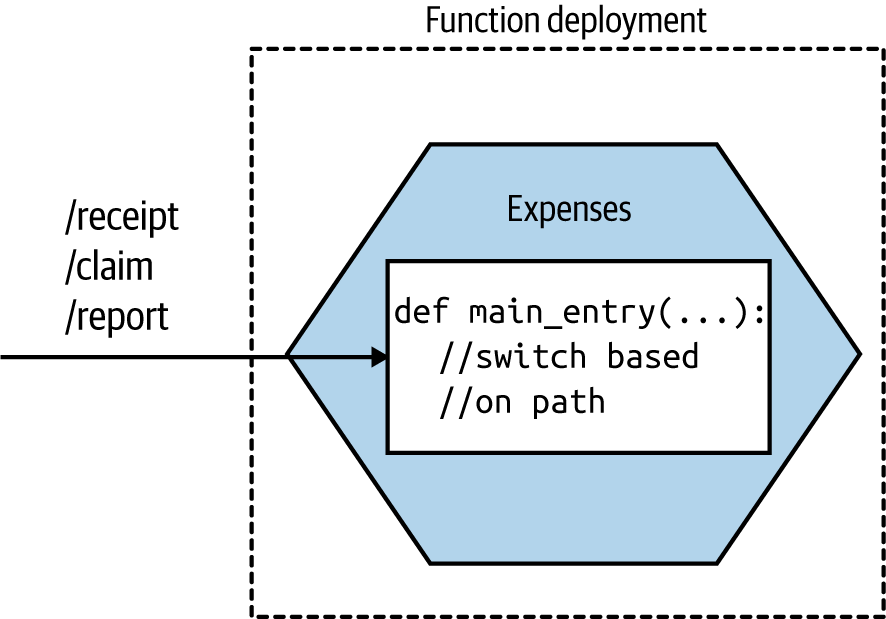
\includegraphics[scale=1]{Pictures/3_single_function.png}
    \caption{Example of Function per microservice.}
    \label{fig:3_single_function}
\end{figure}

In this setup, when the function is invoked, the FaaS platform activates a singular entry point
within the deployed function. This necessitates a mechanism within the function for routing the
invocation to various functionalities that the microservice comprises. For instance, if you have a
microservice like the Expenses service, designed as a REST-based system, it could expose different
endpoints such as /receipt, /claim, or /report. In a single function deployment model, requests to
any of these endpoints are funneled through the same entry point. Consequently, there must be an
internal dispatch system within the function that discerns the path of the incoming request and
directs it to the correct segment of the microservice for processing. This design ensures
streamlined handling of various functionalities within a microservice through a unified FaaS-based
interface\textsuperscript{\cite{microservices_book}}.
\newline
\newline
The \textbf{Function per aggregate} approach adopts a detailed perspective, dividing a single
microservice into several functions, where each function is responsible for a distinct part or
"aggregate" of the microservice's overall role. In this context, an aggregate refers to a group of
domain objects treated as a cohesive unit for the purposes of data manipulation. This approach
aligns well with domain-driven design, where aggregates are typically defined as collections of
objects managed together and often represent real-world entities.

\begin{figure}
    \centering
    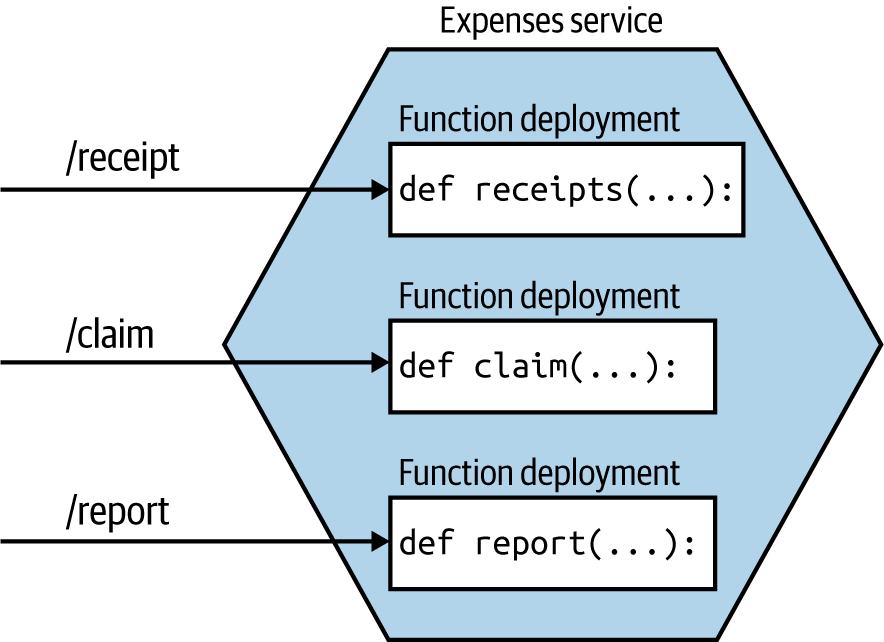
\includegraphics[scale=1]{Pictures/3_multiple_functions.png}
    \caption{Example of Function per aggregate.}
    \label{fig:3_multiple_functions}
\end{figure}

If a microservice manages multiple aggregates, a practical solution is to dedicate a function to
each aggregate, as depicted in figure \ref{fig:3_multiple_functions}. This strategy ensures that all
the logic pertaining to an individual aggregate is encapsulated within a single function. Such an
arrangement simplifies the management and ensures consistent implementation of the aggregate's
life-cycle\textsuperscript{\cite{microservices_book}}. \newline\newline
Adopting this model alters the traditional concept of a microservice instance from a single
deployment unit to a more conceptual framework composed of various functions. These functions,
representing different parts of the microservice, can theoretically be deployed independently. This
not only provides flexibility in deployment but also allows for more granular scaling and
maintenance of the service.

\subsection{Market Overview}
The serverless computing market is poised for rapid expansion, with projections estimating a
compound annual growth rate (CAGR) of 22.2\% from 2024 to 2032, fueled by an escalating demand for
cost-effective computing. Organizations are keen to diminish capital expenditures on IT
infrastructure, and serverless computing meets this need by delivering backend services that only
incur costs when actively used. This pricing model significantly enhances organizational
cost-efficiency and augments scalability, reliability, and the pace of product development to
market\textsuperscript{\cite{serverless_6}}. \newline\newline
Contributing to this growth is a concerted move towards sustainable IT practices, with companies
embracing serverless computing to cut down on IT hardware dependency and improve energy efficiency,
thereby supporting their environmental, social, and governance (ESG) objectives. The adaptability of
serverless computing, compatible with numerous programming environments, is finding traction across
vital sectors like manufacturing, IT, and banking. This is further amplified by the boom in web and
mobile application development, thanks to broader mobile and internet accessibility, where
serverless computing's efficient resource utilization and speedy deployment significantly lower
operational and maintenance costs. Collectively, these factors are making serverless computing a
compelling strategy for organizations seeking to bolster user experiences and maintain a competitive
edge, indicating a strong and dynamic future for the serverless computing
market\textsuperscript{\cite{serverless_6}}.

\newpage

\subsubsection{Trends and Success Rates}

\begin{figure}
    \centering
    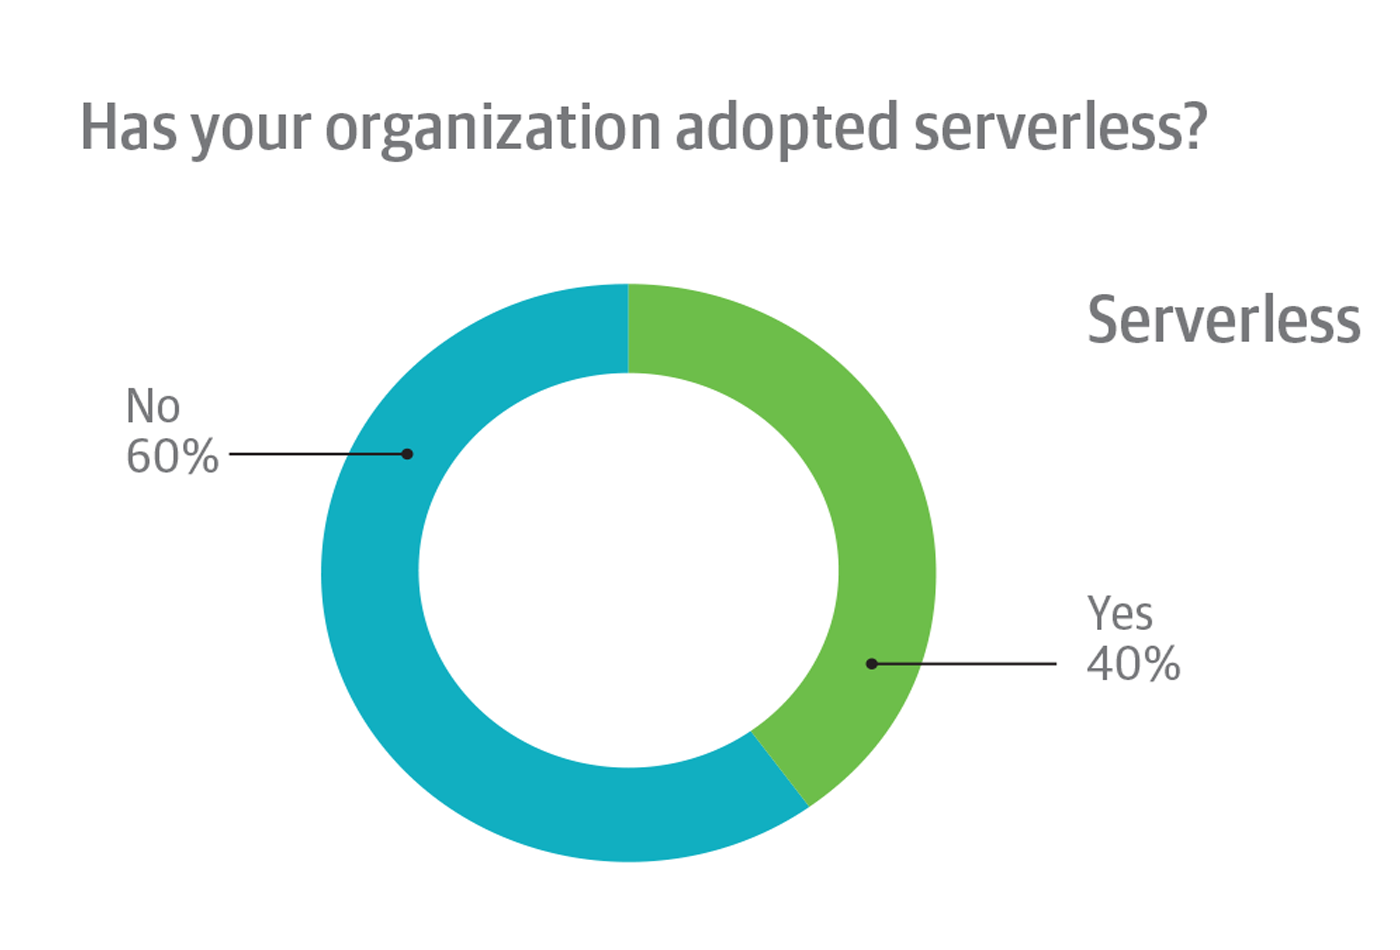
\includegraphics[scale=0.15]{Pictures/3_serverless_adoption.png}
    \caption{Serverless adoption among survey respondents’ organizations.}
    \label{fig:3_serverless_adoption}
\end{figure}

The O'Reilly serverless survey\textsuperscript{\cite{serverless_7}}, with over 1,500 participants,
showcased a high level of engagement with serverless architecture, reflecting its growing
significance in the tech community. The figure \ref{fig:3_serverless_adoption} shows around 40\% of
respondents' organizations had embraced serverless, drawn by the promise of reduced operational
costs and the benefit of automatic scaling. These adopters spanned across various industries and
company sizes, indicating that serverless solutions are not limited to any specific sector or
business scale. The survey also revealed that while a substantial 60\% of organizations had not yet
adopted serverless, the reported benefits and the growing success rates among experienced users
could serve as a catalyst for wider adoption. The benefits driving this interest include not only
cost efficiency and scalability but also the agility to adapt to new business requirements rapidly.

\begin{figure}
    \centering
    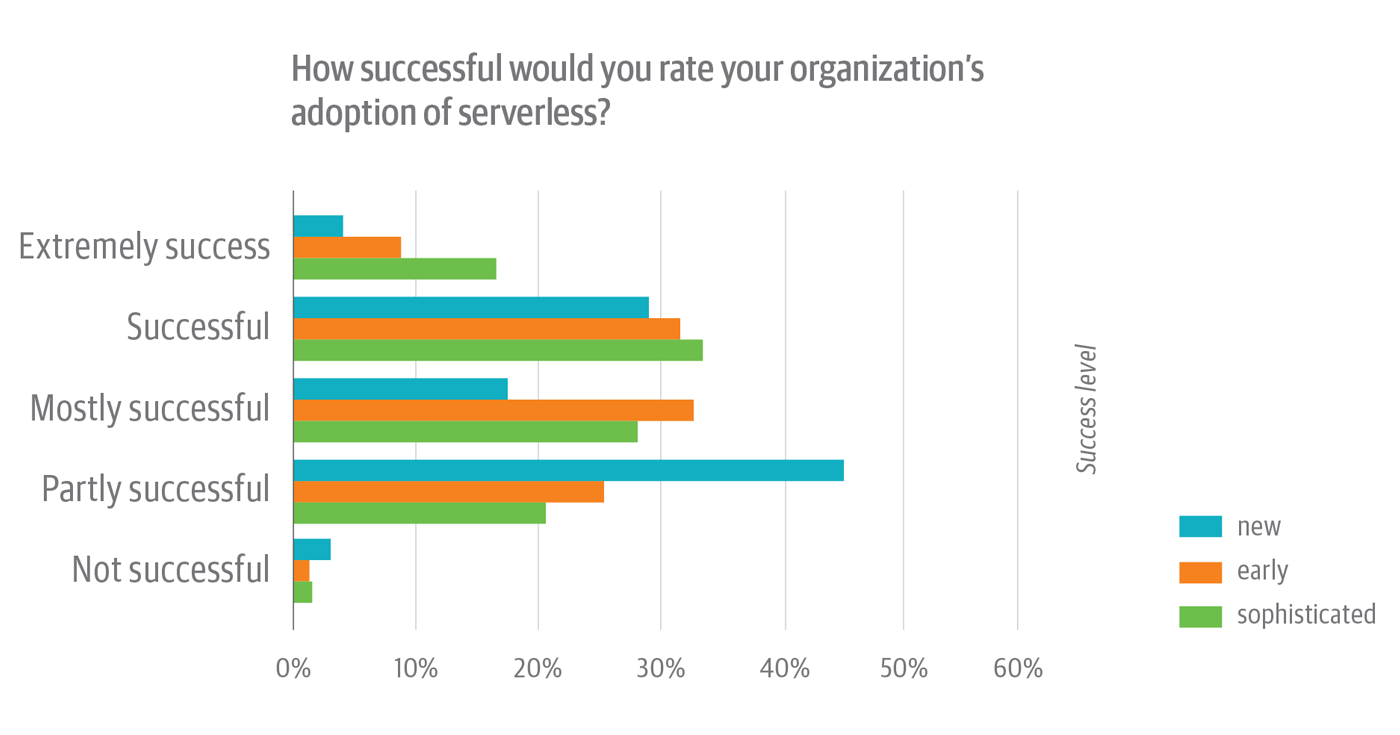
\includegraphics[scale=0.3]{Pictures/3_serverless_adoption_rating.png}
    \caption{Success rating of serverless adoption among survey respondents, broken down by serverless experience level.}
    \label{fig:3_serverless_adoption_rating}
\end{figure}

In figure \ref{fig:3_serverless_adoption_rating} is illustrate how adoption rates varied by
experience, with half of those using serverless for over three years considering their
implementation a success, compared to a lower success rate among newer adopters. This suggests a
correlation between experience with serverless technologies and successful deployment, highlighting
the importance of familiarity and understanding of serverless paradigms in achieving positive
outcomes.
\newline\newline
The data indicates that the serverless model is gaining traction beyond the realm of
early adopters and innovators, with a diverse range of professionals from various fields showing
interest. This is indicative of a broader trend towards infrastructure management models that offer
greater efficiency and flexibility. The survey paints a picture of serverless as a maturing
field with significant potential for growth, as more organizations begin to realize and leverage its
advantages for building modern, scalable, and cost-effective applications.

\subsubsection{Costs}
The cost of using a FaaS model can be lower than using a Software as a Service model, as you only
pay for the specific code you run, rather than paying a monthly or yearly fee for access to the
entire software. Additionally, with a FaaS model, you only pay for the resources that your code
actually uses, like computing time and data storage, rather than paying for the entire server or
infrastructure even when your code is not running. This can result in significant cost savings; it
tends to be more cost-effective than SaaS for short-lived, event-driven workloads as the customer
only pays for the specific computation and resources used by each
function\textsuperscript{\cite{serverless_8}}.
\newline\newline
In this section, we delve into a practical case study drawn from 'Horsa' the company hosting my
thesis research, to illustrate the impact of Enterprise Resource Planning systems in small business
environments. The case involves a small Italian company utilizing Microsoft Business Central, with a
user base of seven employees. By extrapolating this data and applying it to a Function as a Service
environment, we aim to demonstrate the cost-efficiency and potential benefits of embracing FaaS
technology in small-scale business operations. This analysis not only highlights the adaptability
and scalability of FaaS solutions but also presents a tangible example of how transitioning to
cloud-based platforms can offer significant cost savings and operational advantages for small
businesses.

\begin{table}
    \centering
    \begin{tabular}{p{2cm} | p{2.5cm} | p{4.5cm} | p{2.5cm}}
        \hline\hline
        Object     & Usage per day & Conversion                                         & Request/Day \\
        \hline
        Pages      & 3K            & 1 Page = 2 function request 1 to read - 1 to write & 6K          \\
        Report     & 150           & 1 Report = 1 function req.                         & 150         \\
        WebService & 76K           & 1 WS = 1 function req.                             & 76K         \\
        \hline \hline
    \end{tabular}
    \caption{Example of ERP usage}
    \label{tab:3_table_ERP_usage}
\end{table}

Inside the teble \ref{tab:3_table_ERP_usage}, we can see the usage of the ERP system. Now applying
these data to the FaaS cost model.
Considering a month with 26 working days we have:
\begin{equation}
    (150 + 6000 + 76000) * 26 = 2135900 \cong 2.2M \text{ Request per month}
\end{equation}
We will use the FaaS service called Lambda provided by Amazon AWS, prices are calculated based on
the number of calls, duration, and memory allocation for the respective function. By definition,
Lambda functions must be fast and lightweight, so we will use half a second as the duration of each
request and an allocated memory amount of 256 Mb, we will calculate the price not considering the
free plan offered by Amazon:
\begin{equation}
    \text{Total processing time: } 2200000 * 0.5 sec = 1100000.00 sec
\end{equation}
\begin{equation}
    256 \text{ MB} * 0.0009765625 = 0.25 \text{ GB}
\end{equation}
\begin{equation}
    \text{Total processing: } 0.25 \text{ GB} * 1100000.00 sec = 275000 \text{ GB/s}
\end{equation}
\begin{equation}
    \text{Total processing cost: } 275000 \text{ GB/s} * 0.0000195172 \text{ USD} = 5.3672 \text{ USD}
\end{equation}
\begin{equation}
    \text{Request cost: } 2200000 * 0.00000023 \text{ USD} = 0.51 \text{ USD}
\end{equation}
\begin{equation}
    \text{Total monthly lambda cost: }5.3672 \text{ USD} + 0.51 \text{ USD} = 5.88 \text{ USD}
\end{equation}
To this we must also add the cost of the API Gateway for routing requests:
\begin{equation}
    2200000 * 0.00000117 \text{ USD} = 2.57 \text{ USD}
\end{equation}
Finally, the total cost of the enviroment is 8,45 USD per month, that show the flexibility and
cost-effectiveness of the system. This example gives us the reason why the serverless has rapidly
become a popular choice for many organizations, even if the concept is still relatively new.
